\documentclass{beamer}

\usepackage{kotex}
\usepackage{graphicx}
\usepackage{minted}
\usepackage[export]{adjustbox}
\usepackage{textcomp}

\vfuzz=30pt

%%%%%%%%%%%%%%%%%%%%%
%  Beamer Settings  %
%%%%%%%%%%%%%%%%%%%%%
\usetheme[numbering=fraction]{metropolis}
\usecolortheme{rose}
\useoutertheme[subsection=false]{miniframes}

\setbeamertemplate{itemize item}[square]
\setbeamertemplate{itemize subitem}[triangle]
\setbeamertemplate{itemize subsubitem}[circle]

%%%%%%%%%%%%%%%%%%%
%  Font Settings  %
%%%%%%%%%%%%%%%%%%%
\usepackage[factor=500]{microtype}

\usepackage[mathrm=sym]{unicode-math}

\setmainfont{TeXGyrePagellaX}
\setsansfont{Roboto}[
  BoldFont = *-Medium,
  BoldItalicFont = *-MediumItalic
]
\setmonofont{Inconsolata}

\setmainhangulfont{NanumMyeongjo}
\setsanshangulfont{NanumGothic}[AutoFakeSlant=0.18]

\setmathfont{Fira Math}
\setmathfont{Fira Sans Medium}[range=bfsfup]
\setmathfont{Fira Sans Medium Italic}[range=bfsfit]
\setmathfont{STIX Two Math}[range=cal]

%%%%%%%%%%%%%%%%%%%%%
%  Minted Settings  %
%%%%%%%%%%%%%%%%%%%%%
\renewcommand\theFancyVerbLine{\textsf{\tiny\arabic{FancyVerbLine}}}

\newminted{latex}{
  escapeinside=||,
  mathescape,
  autogobble,
  linenos,
  breaklines,
  numbersep=5pt,
  frame=single,
  fontsize=\scriptsize}
\newmintinline[ltxverb]{latex}{escapeinside=||}

%%%%%%%%%%%%%%%%%%%%%%%
% Custom Settings  %
%%%%%%%%%%%%%%%%%%%%%%%
\def\tbs{\textbackslash}

%%%%%%%%%%%%%%%%%%%%%%%
%  Document Settings  %
%%%%%%%%%%%%%%%%%%%%%%%

\title{%
  {\large memoir와 expl3로 해보는 Book Design}\\
  Chapter Style
}

\author{이재호}
\institute{memoir 스터디 그룹}
\date{\today}

%%%%%%%%%%%%%%
%  Document  %
%%%%%%%%%%%%%%
\begin{document}

\maketitle

\section{Overview}

% \begin{frame}[fragile]{문서의 챕터}
% \end{frame}

\begin{frame}[fragile]{\texttt{\textbackslash chapter}가 하는 일}
  memoir에서 챕터 모양을 바꾸기 위해서는 \ltxverb/\chapterstyle{|<style>|}/ 사용

  \pause
  일반적으로 \LaTeX에서는 \ltxverb/\@makechapterhead/로 \ltxverb/\chapter/의
  서식을 지정, \ltxverb/\@makeschapterhead/로 \ltxverb/\chapter*/의 서식을 지정

  \pause
  memoir에서는 대략...
  \begin{columns}[T]
    \begin{column}{0.5\textwidth}
      \begin{latexcode}
        % \chapter with secnumdepth $\geq$ 0
        \chapterheadstart
        \printchaptername \chapternamenum \printchapternum
        \afterchapternum
        \printchaptertitle{The title}
        \afterchaptertitle
      \end{latexcode}
    \end{column}

    \begin{column}{0.5\textwidth}
      \begin{latexcode}
        % \chapter* with secnumdepth < 0
        \chapterheadstart
        \printchapternonum
        \printchaptertitle{The title}
        \afterchaptertitle
      \end{latexcode}
    \end{column}
  \end{columns}
\end{frame}

\begin{frame}[fragile]{\texttt{\textbackslash chapterstyle}이 하는 일}
  매 chapter style 마다, 다음과 같은 매크로들이 초기화된다:
  \begin{latexcode}
    \renewcommand\chapterheadstart{\vspace*{\beforechapskip}}
    \renewcommand\printchaptername{\chapnamefont \@chapapp}
    \renewcommand\chapternamenum{\space}
    \renewcommand\printchapternum{\chapnumfont \thechapter}
    \renewcommand\afterchapternum{\par\nobreak\vskip \midchapskip}
    \renewcommand\printchapternonum{}
    \renewcommand\printchaptertitle[1]{\chaptitlefont #1}
    \renewcommand\afterchaptertitle{\par\nobreak\vskip \afterchapskip}
  \end{latexcode}

  \pause
  마지막으로, \ltxverb/\makechapterstyle{|<style>|}{|<code>|}/를 통해 새로운
  chapter style을 정의할 수 있다.

  이를 사용하려면, \ltxverb/\chapterstyle{|<name>|}/을 사용한다.
\end{frame}


\section{명령어 분석}

\begin{frame}[fragile]
  {\texttt{\tbs openright}, \texttt{\tbs openleft}, \texttt{\tbs openany} 분석}
  \begin{description}
    \item[openright] 챕터 헤딩이 직후 우측 페이지에 위치한다.
    \item[openleft] 챕터 헤딩이 직후 좌측 페이지에 위치한다.
    \item[openany] 챕터 헤딩이 직후 페이지에 위치한다.
  \end{description}

  또한 \ltxverb/\openright/와 같이 문서 아무 곳에서 사용하면 설정이 바뀐다.

  \pause
  이는 다음과 같은 일을 하도록 정의되어 있다:
  \begin{latexcode}
    \newcommand{\openright}{\@openrighttrue\@openleftfalse%
      \gdef\clearforchapter{\cleartorecto}}
    \newcommand{\openany}{\@openrightfalse\@openleftfalse%
      \gdef\clearforchapter{\clearpage}}
    \newcommand{\openleft}{\@openlefttrue
      \gdef\clearforchapter{\cleartoverso}}
  \end{latexcode}
\end{frame}

\begin{frame}[fragile]{\texttt{\tbs clearforchapter} 분석}
  직전에 소개된 \ltxverb/\openright/, \ltxverb/\openleft/, \ltxverb/\openany/에
  의해 설정된다.

  만약 이를 새로 정의한다면 챕터가 시작되기 직전에 해야하는 작업을 수행할 수
  있다.
\end{frame}

\begin{frame}[fragile]{\texttt{\tbs clearforchapter} 예시}
  \begin{latexcode}
    \renewcommand*{\clearforchapter}{}
  \end{latexcode}

  \begin{columns}
    \begin{column}{0.4\textwidth}
      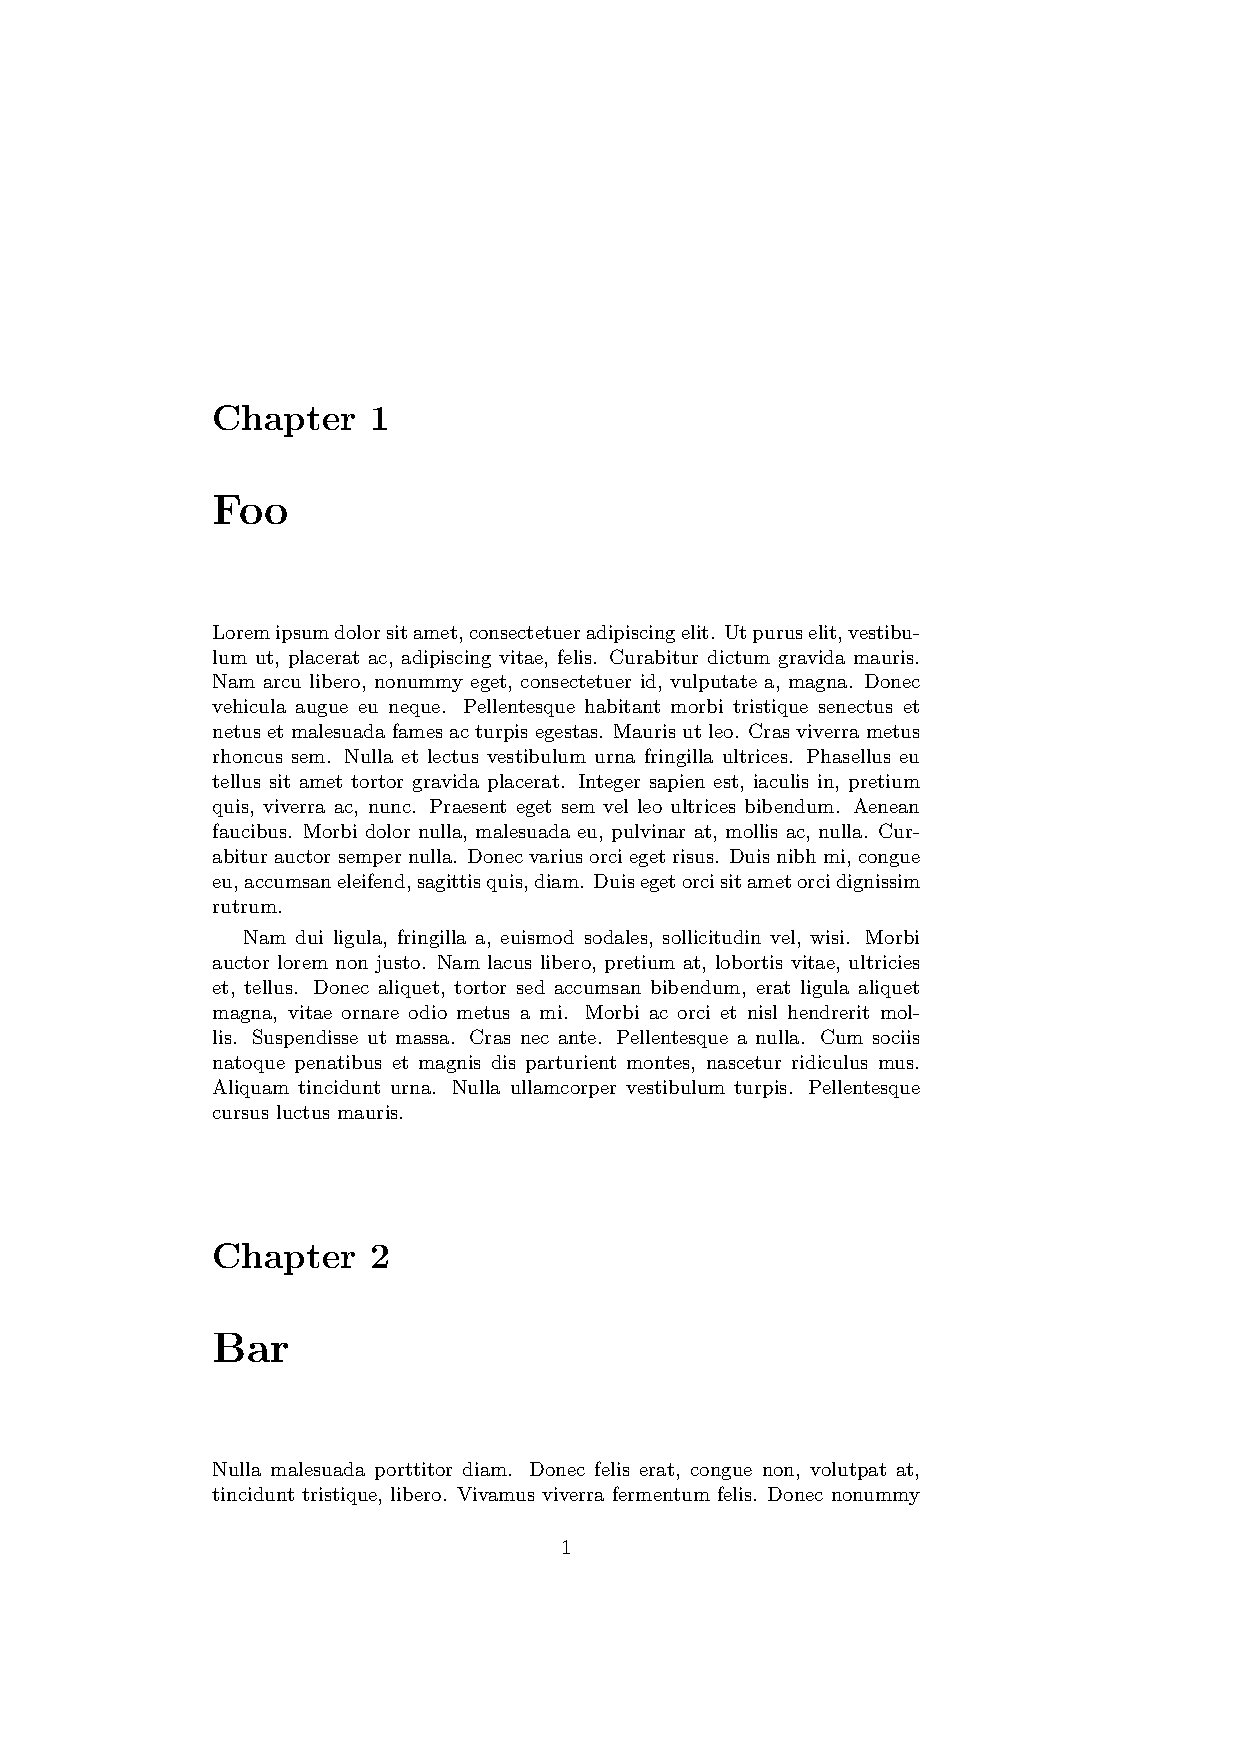
\includegraphics[frame,page=1,width=\linewidth]{examples/clearforchapter}
    \end{column}
    \begin{column}{0.4\textwidth}
      \includegraphics[frame,page=2,width=\linewidth]{examples/clearforchapter}
    \end{column}
  \end{columns}
\end{frame}

\begin{frame}[fragile]{\texttt{\tbs memendofchapterhook} 분석}
  \ltxverb/\clearforchapter/가 챕터 시작 직전에 실행된다면,
  \ltxverb/\memendofchapterhook/은 챕터의 맨 끝에서 실행된다.

  기본적으로는 아무것도 하지 않도록 정의되어 있다.
\end{frame}

\begin{frame}[fragile]{\texttt{\tbs memendofchapterhook} 예시}
  \begin{columns}
    \begin{column}{0.6\textwidth}
      \begin{latexcode}
        % \usepackage{amssymb}
        \renewcommand*{\clearforchapter}{}
        \renewcommand{\memendofchapterhook}{%
          \begin{center}
            $\lozenge\lozenge\lozenge$
          \end{center}}
      \end{latexcode}
    \end{column}

    \begin{column}{0.4\textwidth}
      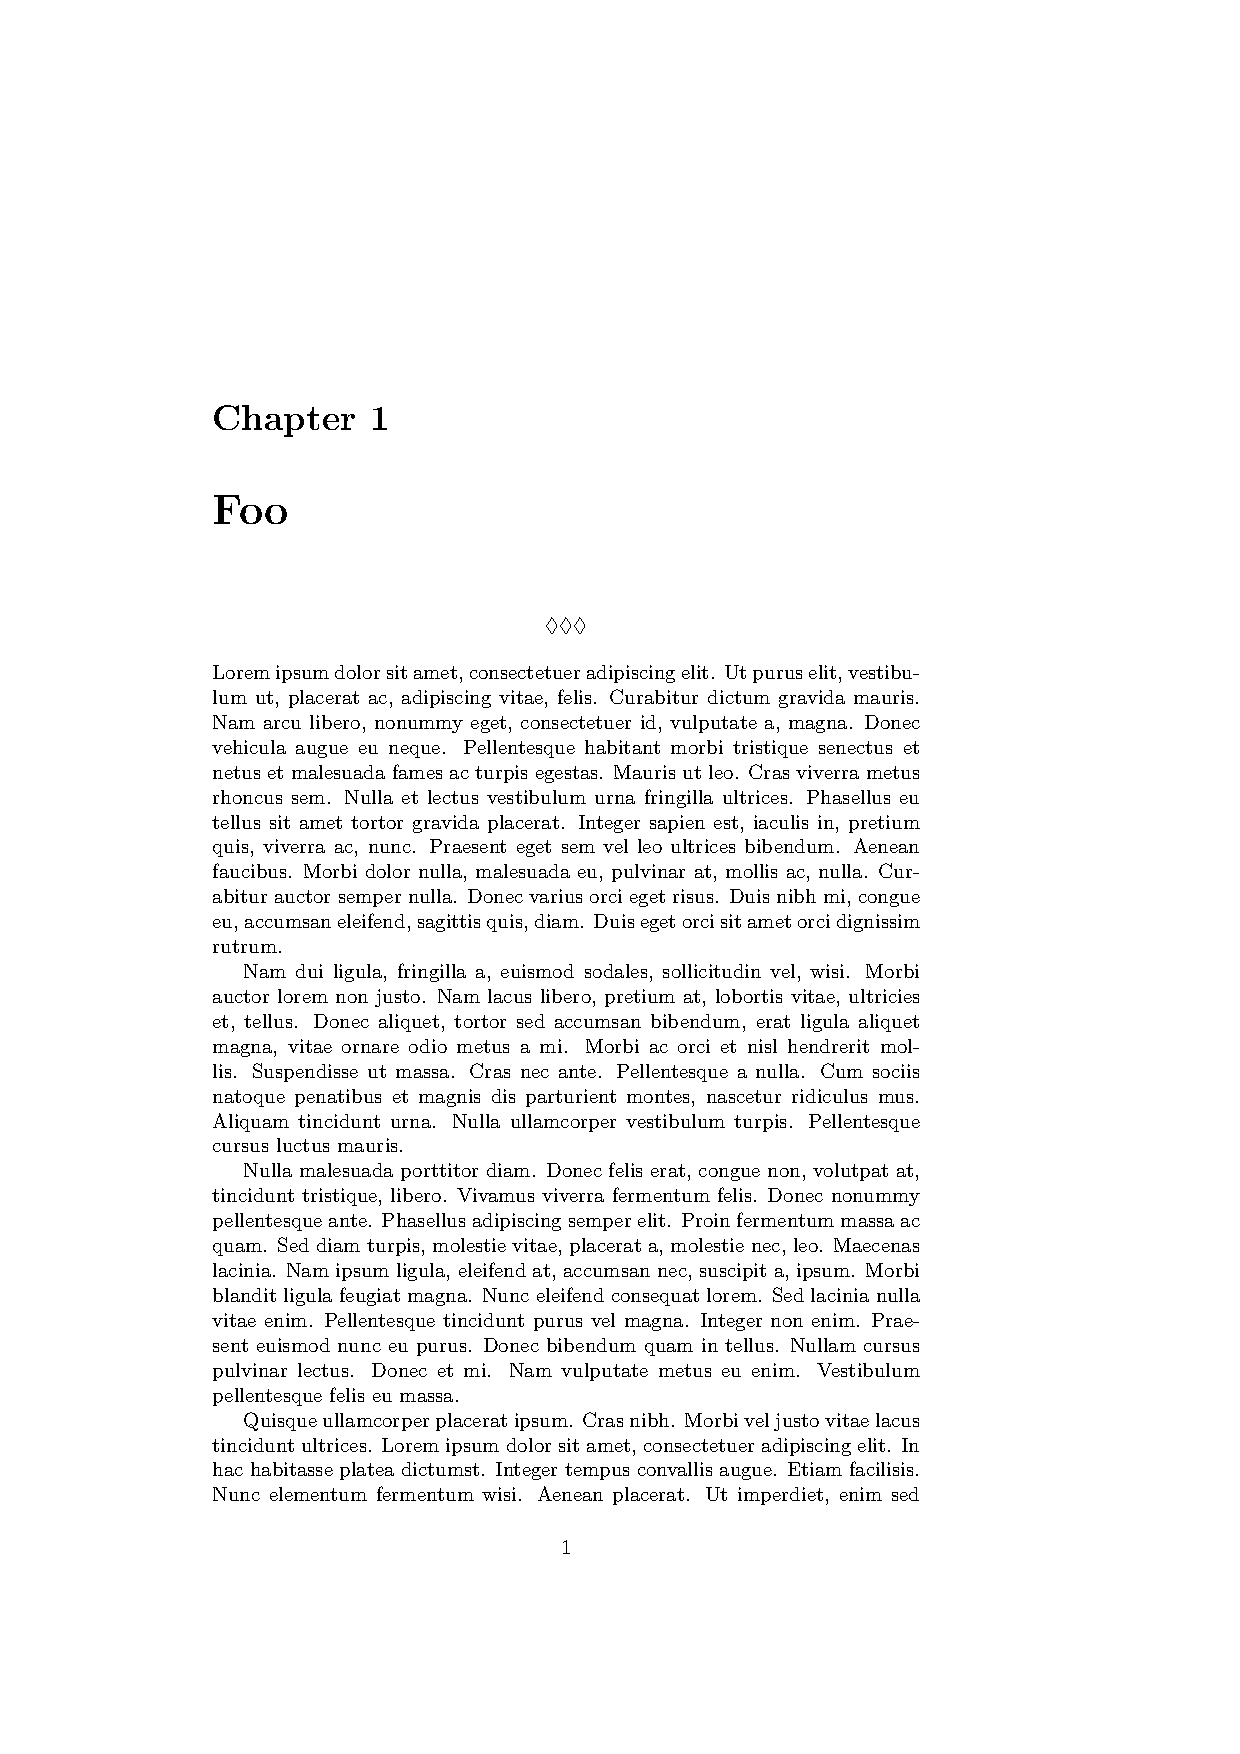
\includegraphics[frame,page=1,width=\linewidth]{examples/memendofchapterhook}
    \end{column}
  \end{columns}
\end{frame}

\begin{frame}[fragile]
  {\texttt{\tbs chapterheadstart}와 \texttt{\tbs beforechapskip} 분석}
  \ltxverb/\chapterheadstart/은 챕터 제목과 번호를 출력하기 직전에 실행되며,
  기본적으로는 50pt로 설정되어 있는 \ltxverb/\beforechapskip/을 출력한다.
\end{frame}

\begin{frame}[fragile]
  {\texttt{\tbs chapterheadstart}와 \texttt{\tbs beforechapskip} 예시}
  \begin{overprint}
    \onslide<1>
    \begin{columns}
      \begin{column}{0.5\textwidth}
        \begin{latexcode}
          \setlength\beforechapskip{50pt}
        \end{latexcode}
        \begin{center}
          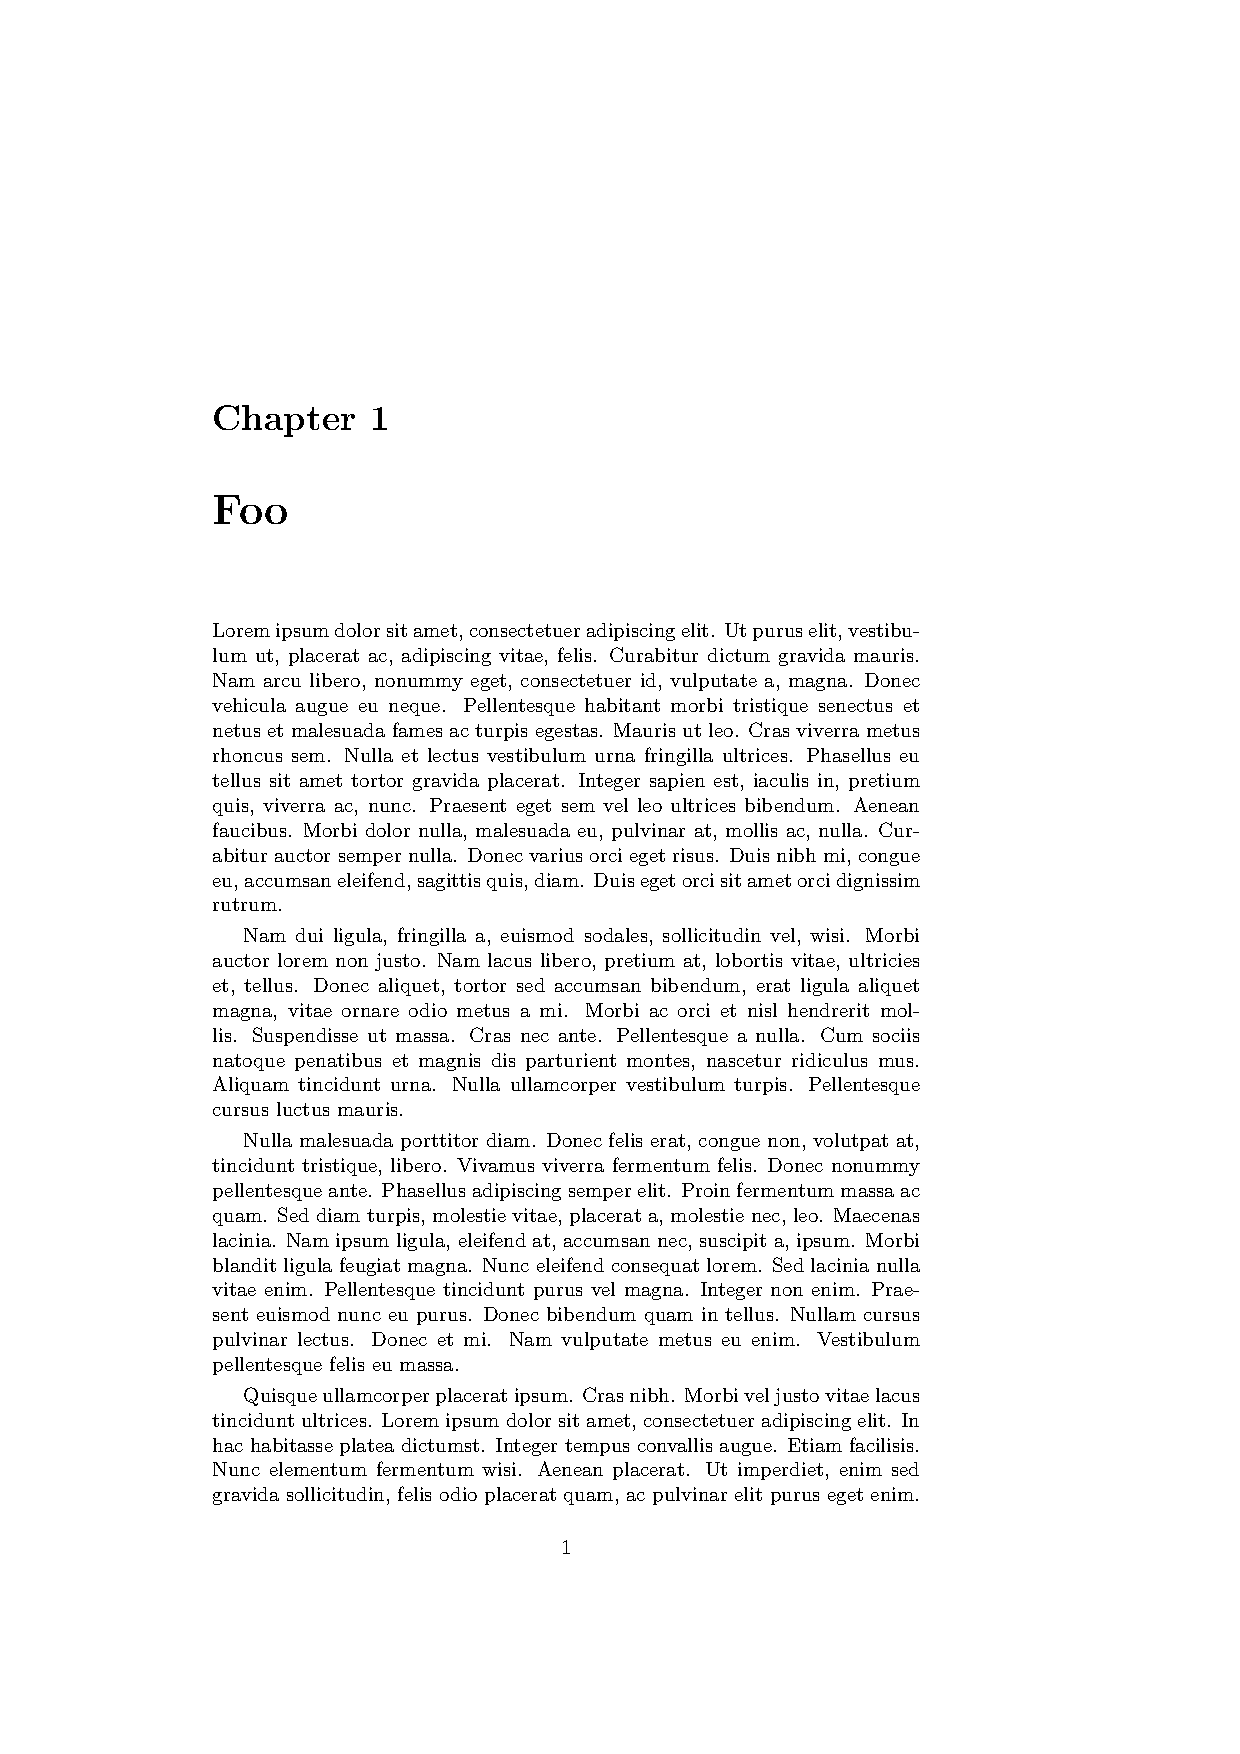
\includegraphics[frame,page=1,width=0.8\linewidth]{examples/chapterheadstart}
        \end{center}
      \end{column}

      \begin{column}{0.5\textwidth}
        \begin{minted}[mathescape,
                       autogobble,
                       linenos,
                       numbersep=5pt,
                       frame=single,
                       fontsize=\scriptsize]{latex}
          \setlength\beforechapskip{-\baselineskip}
        \end{minted}
        \begin{center}
          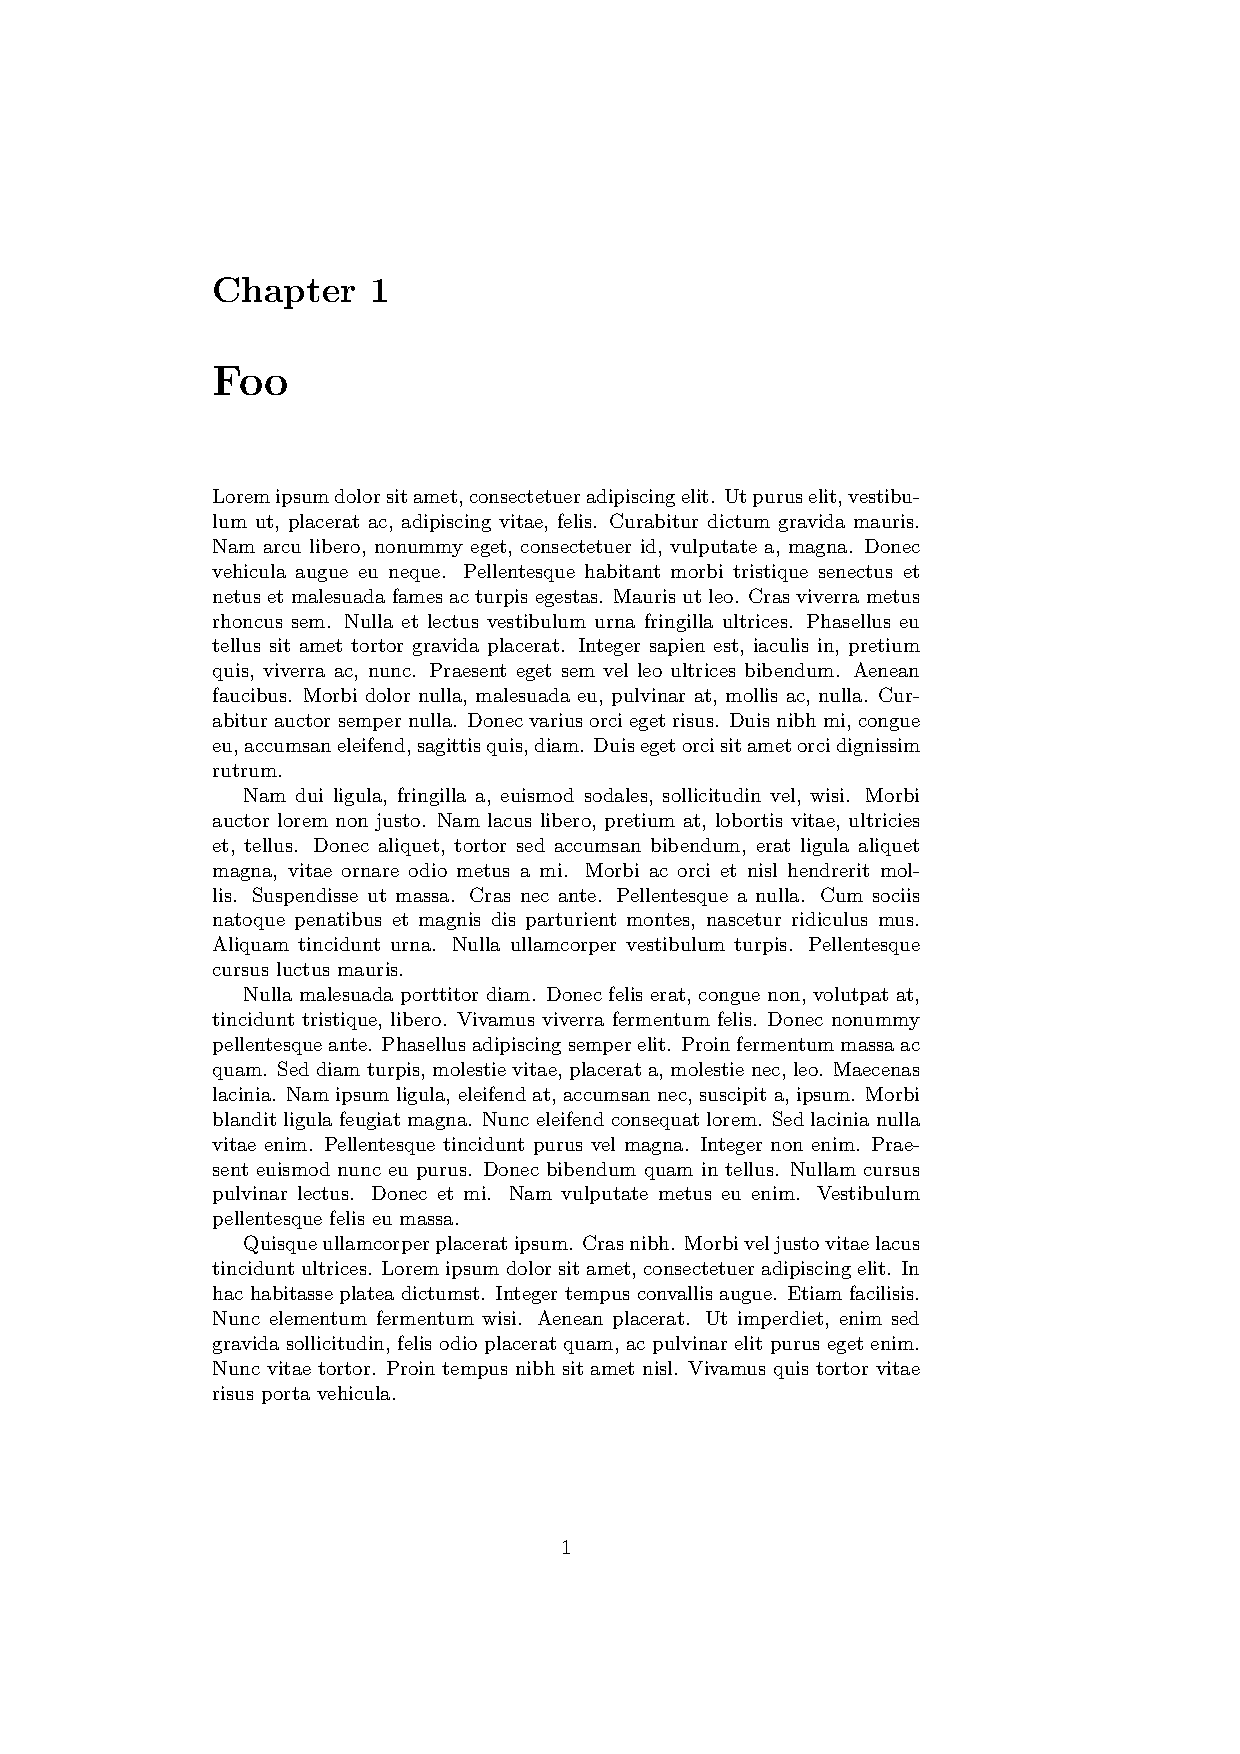
\includegraphics[frame,page=1,width=0.8\linewidth]{examples/chapterheadstart-2}
        \end{center}
      \end{column}
    \end{columns}

    \onslide<2>
    \begin{columns}
      \begin{column}{0.5\textwidth}
        \begin{latexcode}
          \setlength\beforechapskip{50pt}
        \end{latexcode}
        \begin{center}
          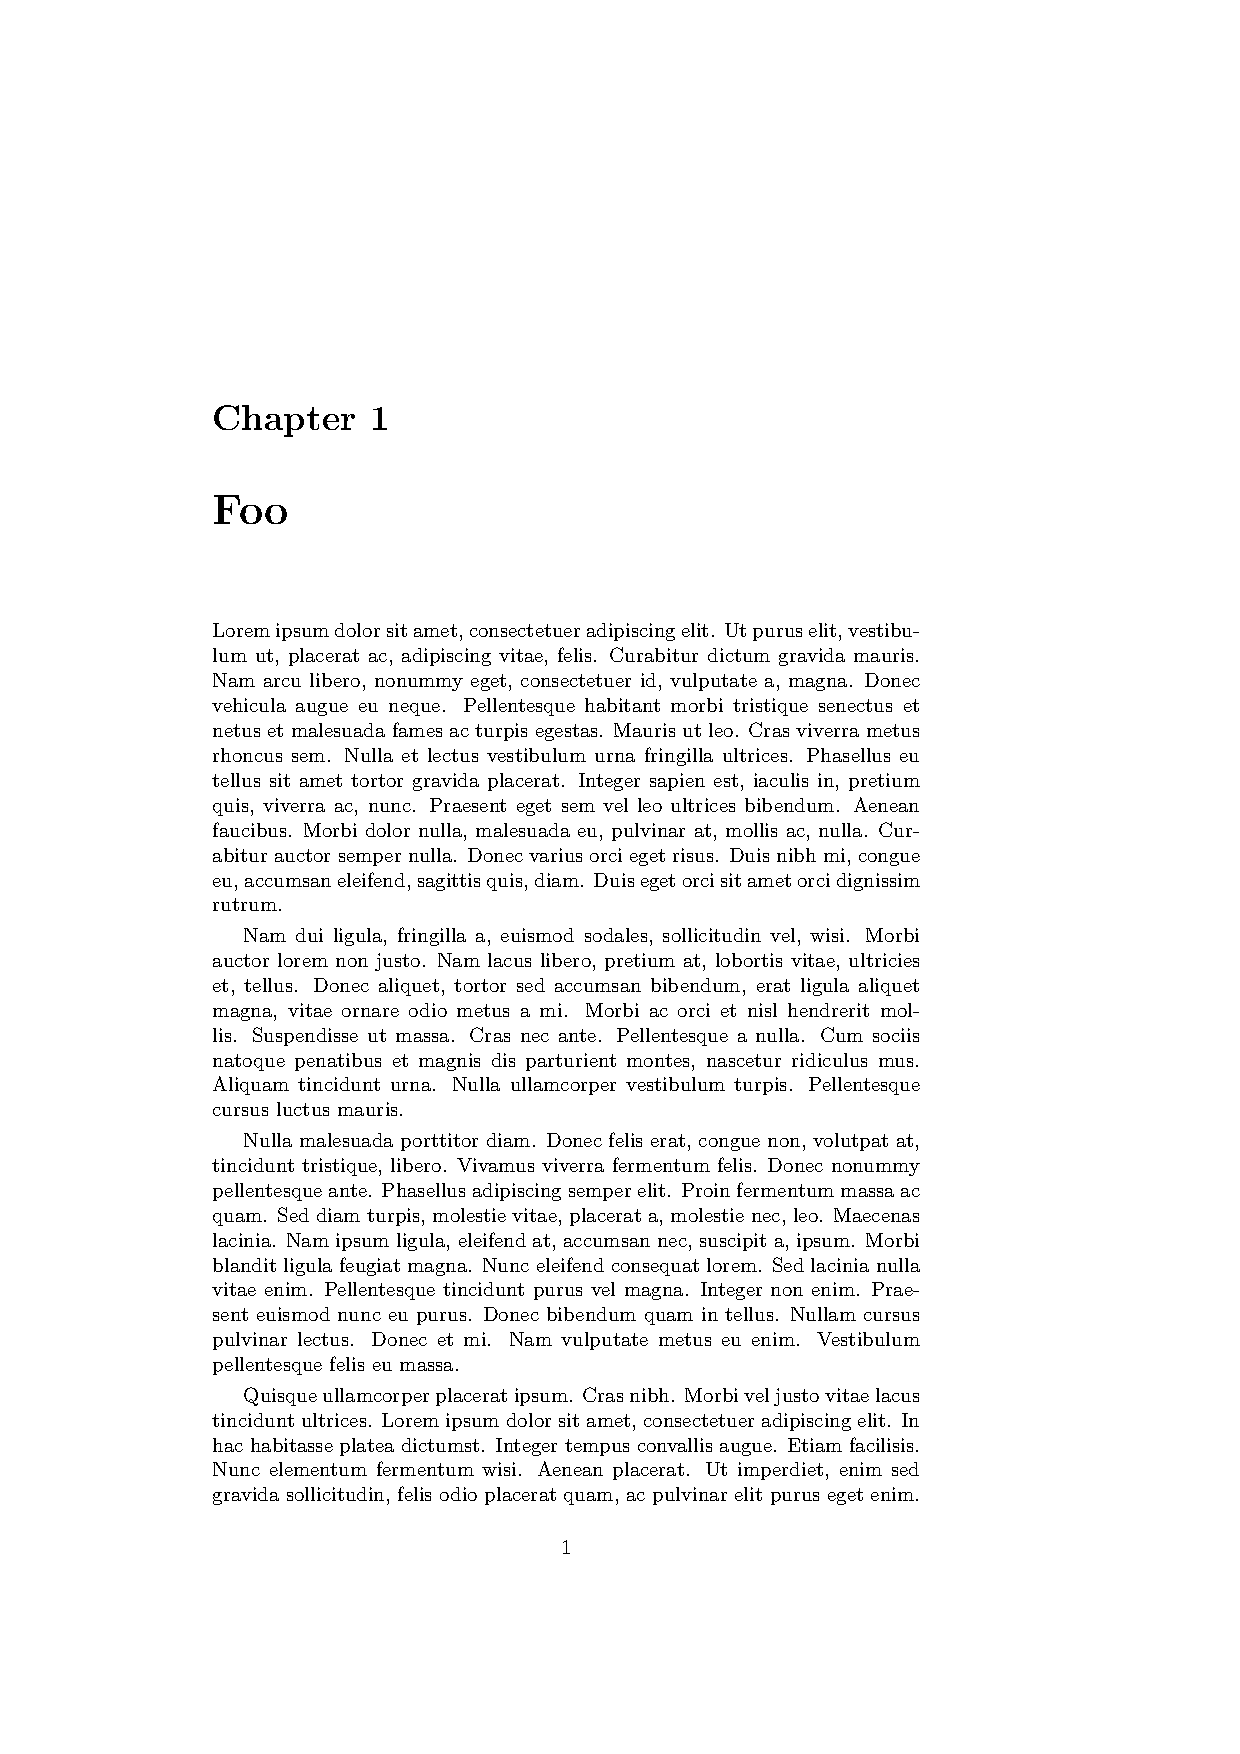
\includegraphics[frame,page=1,width=0.8\linewidth]{examples/chapterheadstart}
        \end{center}
      \end{column}

      \begin{column}{0.5\textwidth}
        \begin{latexcode}
          \renewcommand*{\chapterheadstart}{}
        \end{latexcode}
        \begin{center}
          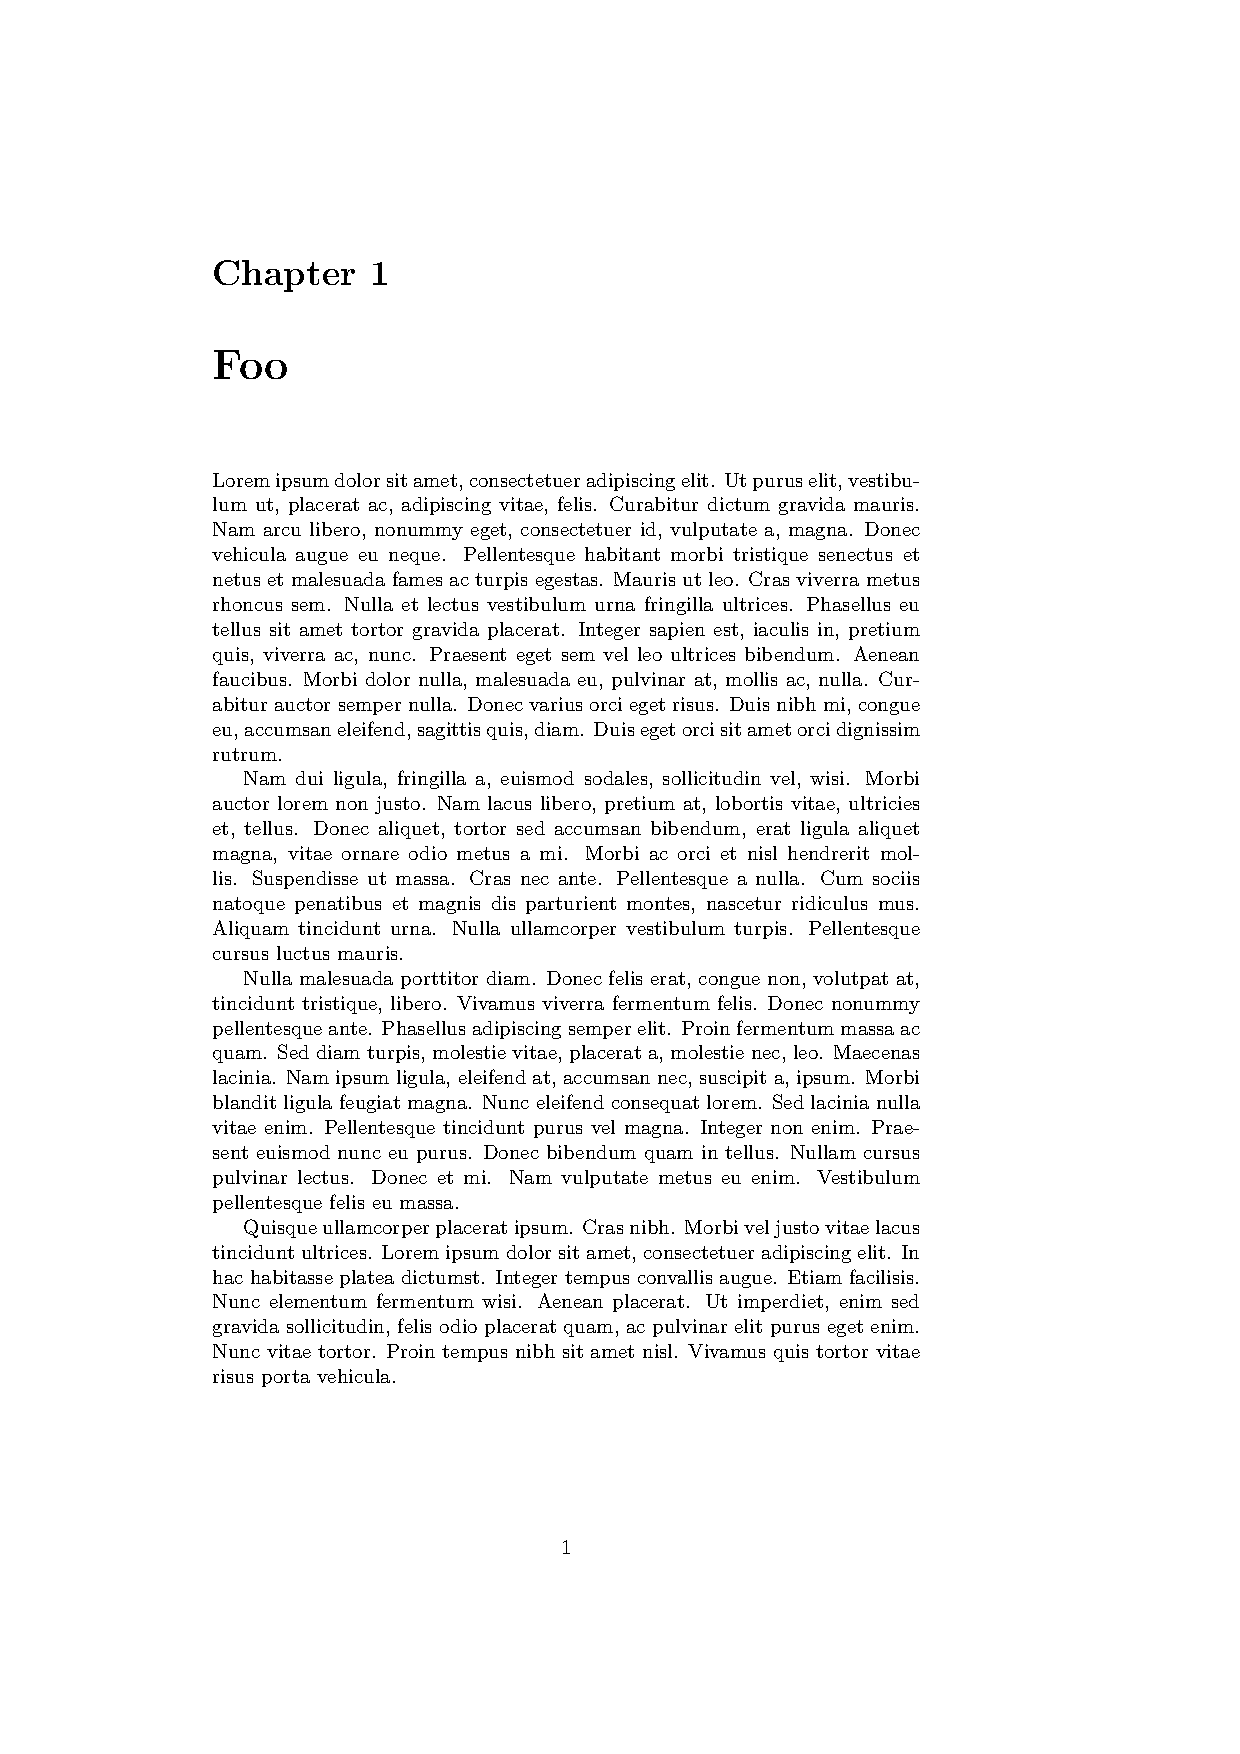
\includegraphics[frame,page=1,width=0.8\linewidth]{examples/chapterheadstart-3}
        \end{center}
      \end{column}
    \end{columns}
  \end{overprint}
\end{frame}

\begin{frame}[fragile]
  {\texttt{\tbs afterchapternum}과 \texttt{\tbs midchapskip} 분석}
  \ltxverb/\afterchapternum/은 챕터 번호를 출력한 직후에 실행되며, 기본적으로는
  20pt로 설정되어 있는 \ltxverb/\midchapskip/을 출력한다.
\end{frame}

\begin{frame}[fragile]
  {\texttt{\tbs afterchapternum}과 \texttt{\tbs midchapskip} 예시}
  \begin{overprint}
    \onslide<1>
    \begin{columns}
      \begin{column}{0.5\textwidth}
        \begin{latexcode}
          \setlength\midchapskip{20pt}
        \end{latexcode}
        \begin{center}
          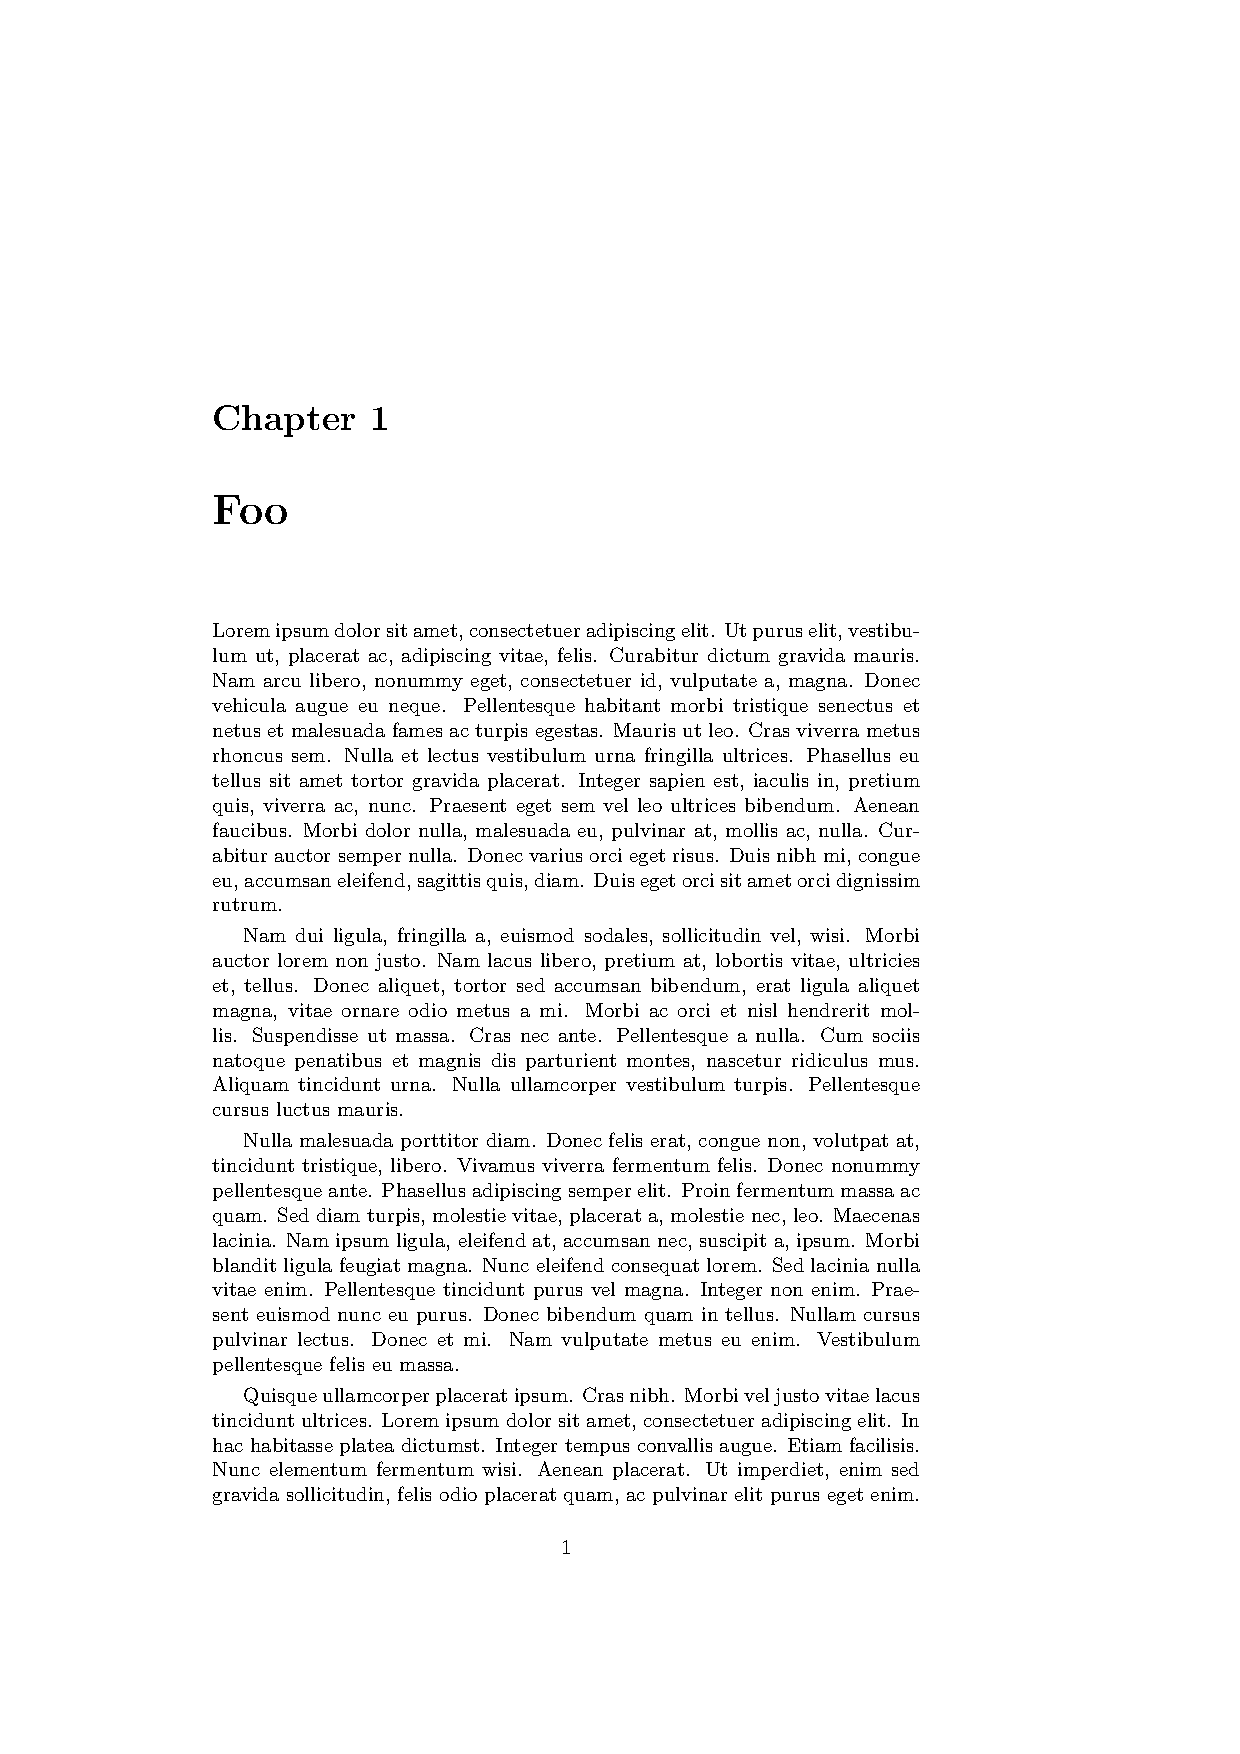
\includegraphics[frame,page=1,width=0.8\linewidth]{examples/afterchapternum}
        \end{center}
      \end{column}

      \begin{column}{0.5\textwidth}
        \begin{latexcode}
          \setlength\midchapskip{0pt}
        \end{latexcode}
        \begin{center}
          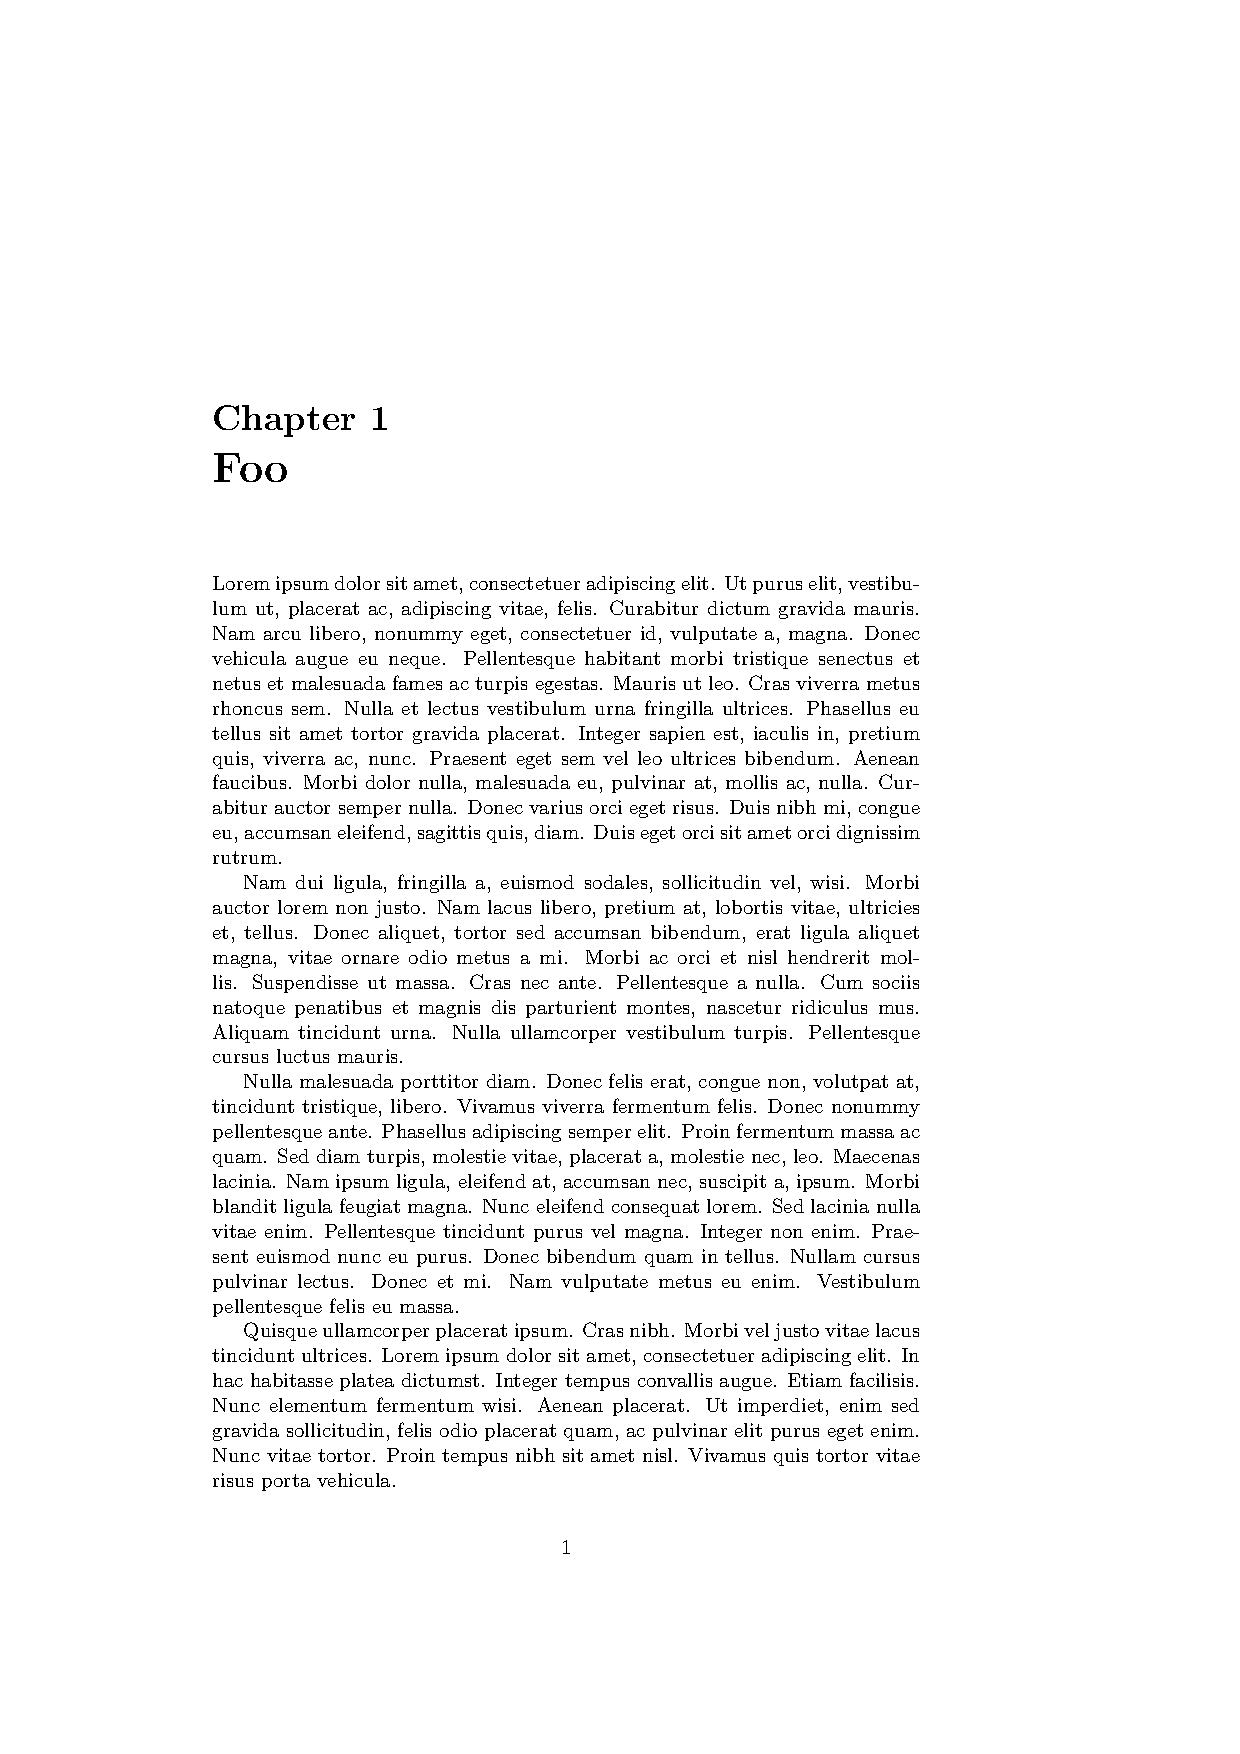
\includegraphics[frame,page=1,width=0.8\linewidth]{examples/afterchapternum-2}
        \end{center}
      \end{column}
    \end{columns}

    \onslide<2>
    \begin{columns}
      \begin{column}{0.5\textwidth}
        \begin{latexcode}
          \setlength\midchapskip{20pt}
        \end{latexcode}
        \begin{center}
          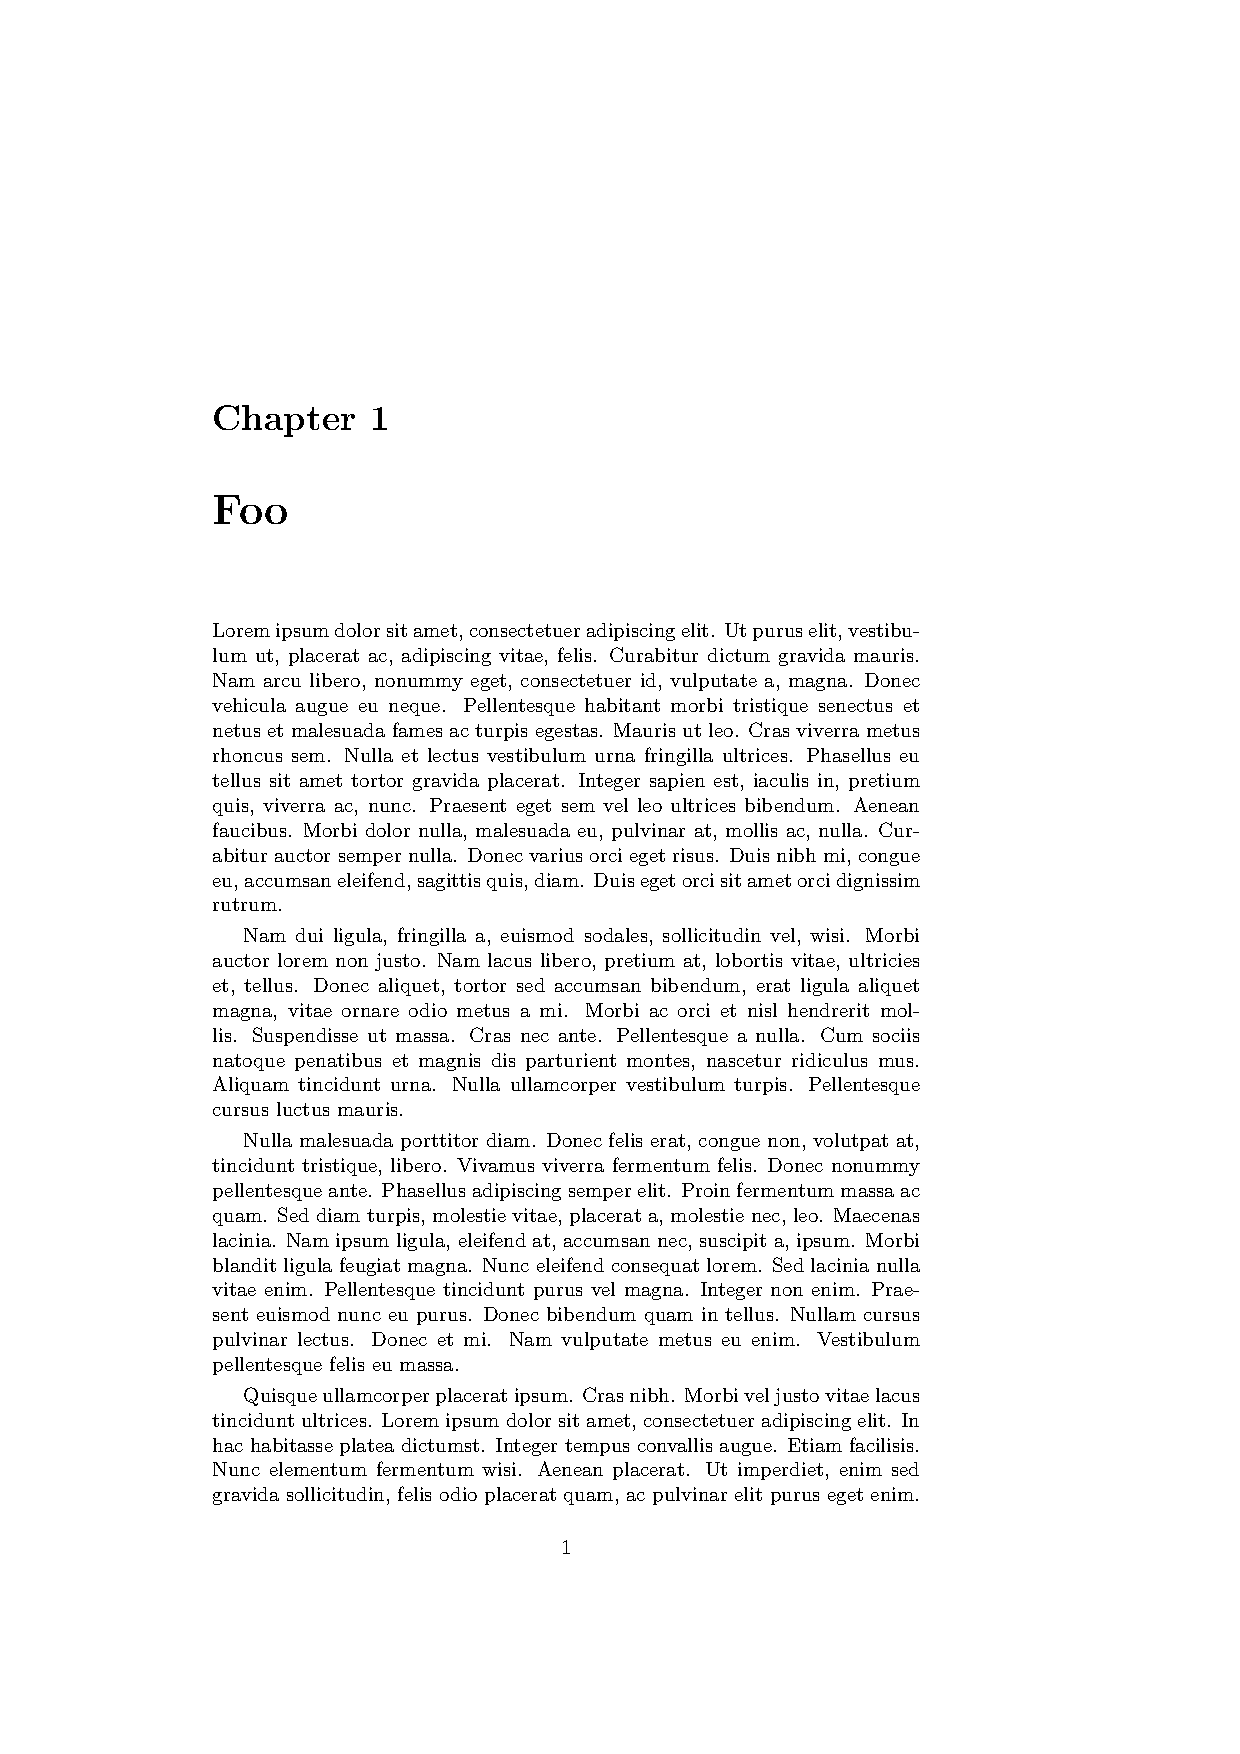
\includegraphics[frame,page=1,width=0.8\linewidth]{examples/afterchapternum}
        \end{center}
      \end{column}

      \begin{column}{0.5\textwidth}
        \begin{minted}[mathescape,
                       escapeinside=||,
                       autogobble,
                       linenos,
                       numbersep=5pt,
                       frame=single,
                       fontsize=\tiny]{latex}
          \renewcommand*{\afterchapternum}{\par\nobreak\vskip 0pt}|\vphantom{\LARGE a}|
        \end{minted}
        \begin{center}
          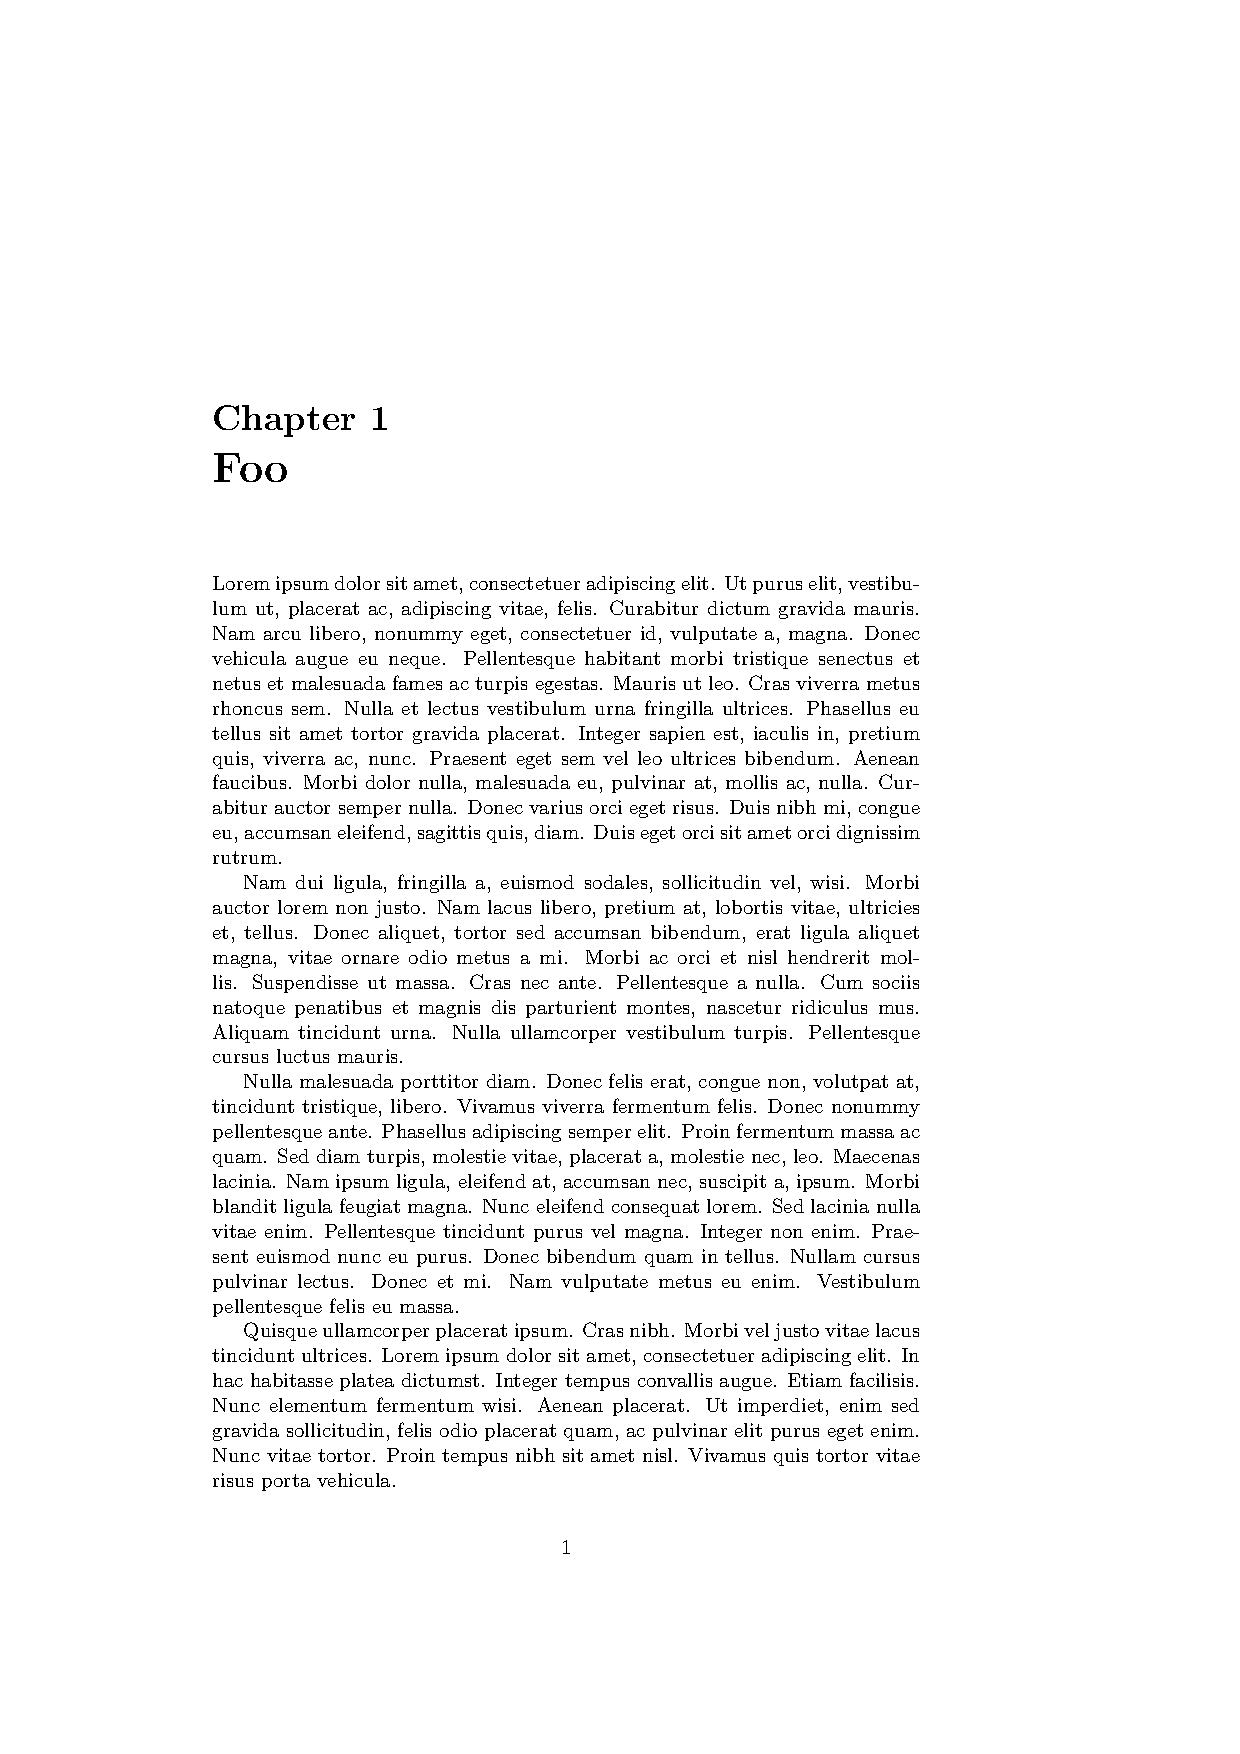
\includegraphics[frame,page=1,width=0.8\linewidth]{examples/afterchapternum-3}
        \end{center}
      \end{column}
    \end{columns}
  \end{overprint}
\end{frame}

\begin{frame}[fragile]
  {\texttt{\tbs afterchaptertitle}과 \texttt{\tbs afterchapskip} 분석}
  \ltxverb/\afterchaptertitle/은 챕터 제목을 출력한 직후에 실행되며,
  기본적으로는 40pt로 설정되어 있는 \ltxverb/\afterchapskip/을 출력한다.
\end{frame}

\begin{frame}[fragile]
  {\texttt{\tbs afterchaptertitle}과 \texttt{\tbs afterchapskip} 예시}
  \begin{overprint}
    \onslide<1>
    \begin{columns}
      \begin{column}{0.5\textwidth}
        \begin{latexcode}
          \setlength\afterchapskip{40pt}
        \end{latexcode}
        \begin{center}
          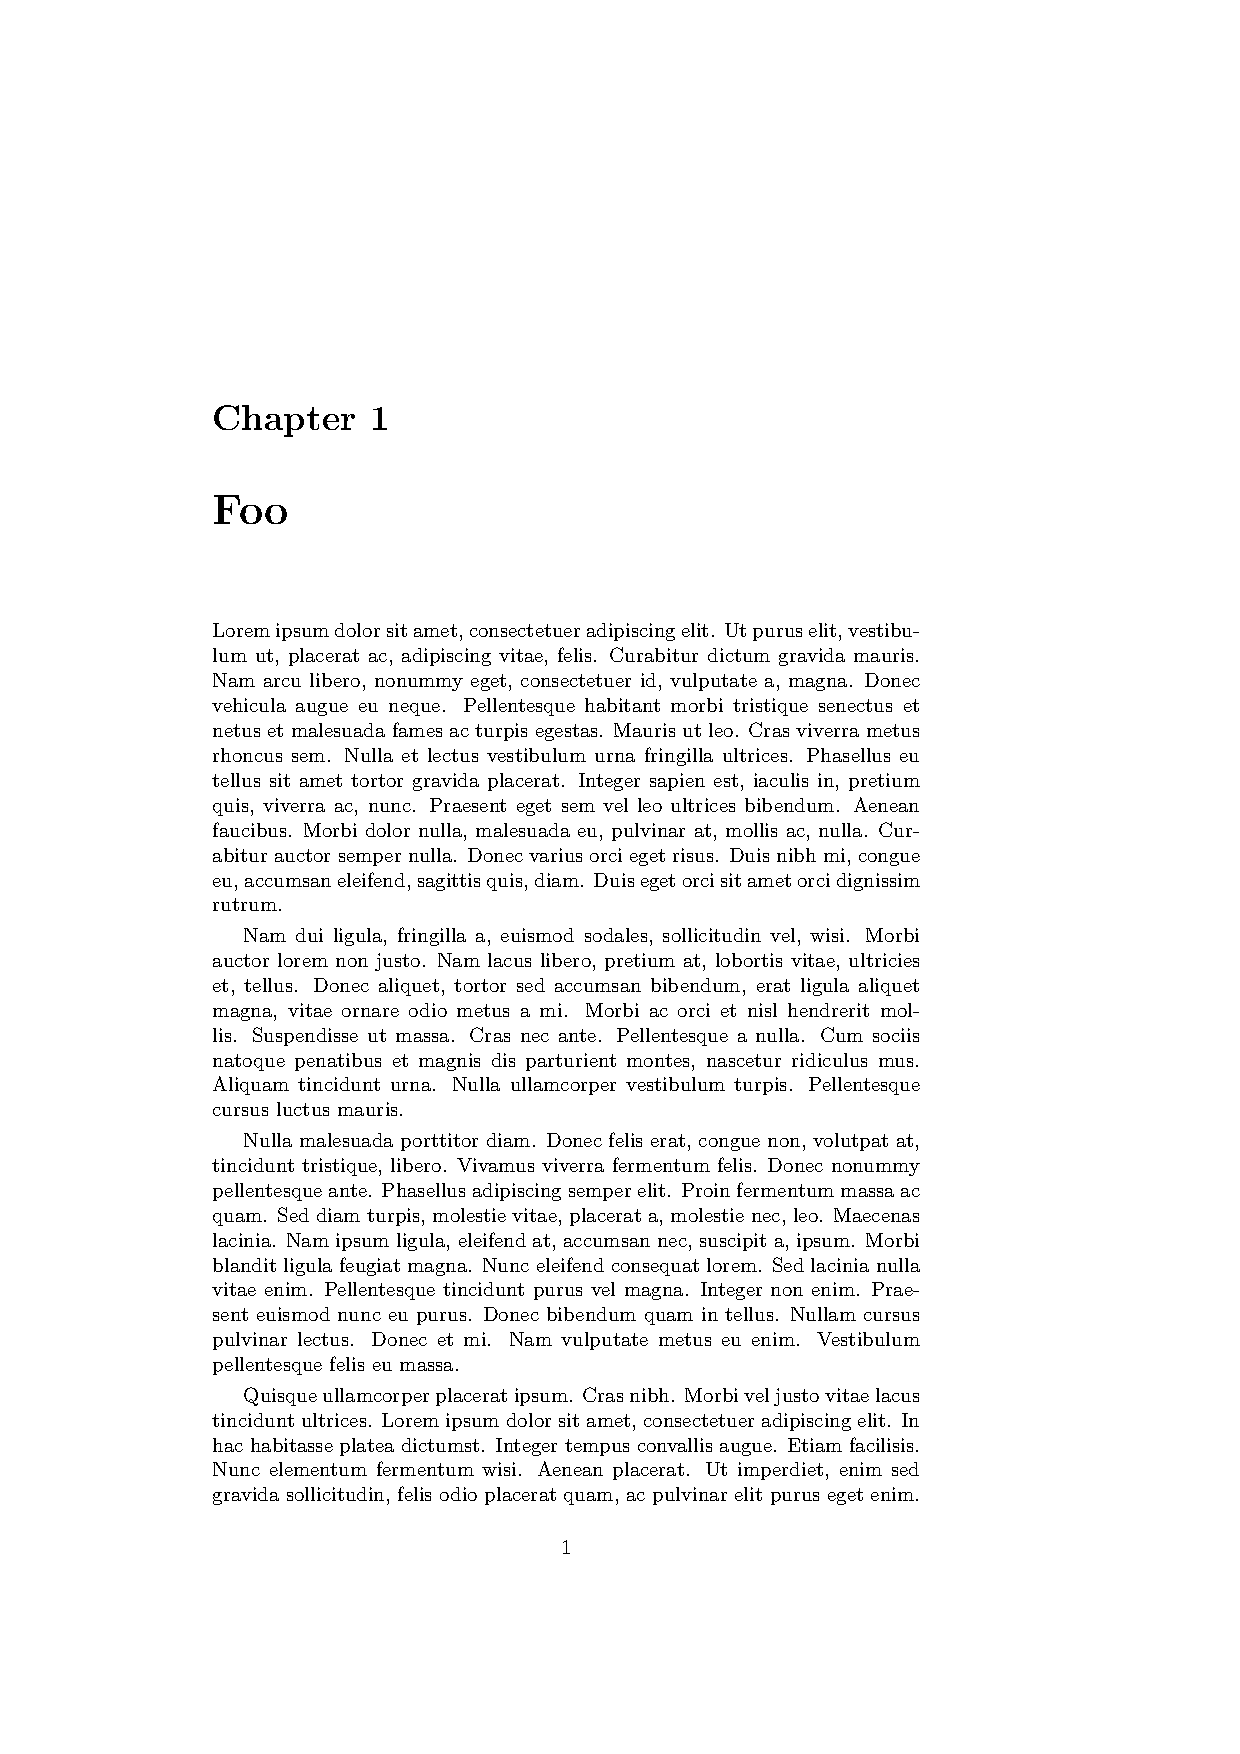
\includegraphics[frame,page=1,width=0.8\linewidth]{examples/afterchaptertitle}
        \end{center}
      \end{column}

      \begin{column}{0.5\textwidth}
        \begin{latexcode}
          \setlength\afterchapskip{0pt}
        \end{latexcode}
        \begin{center}
          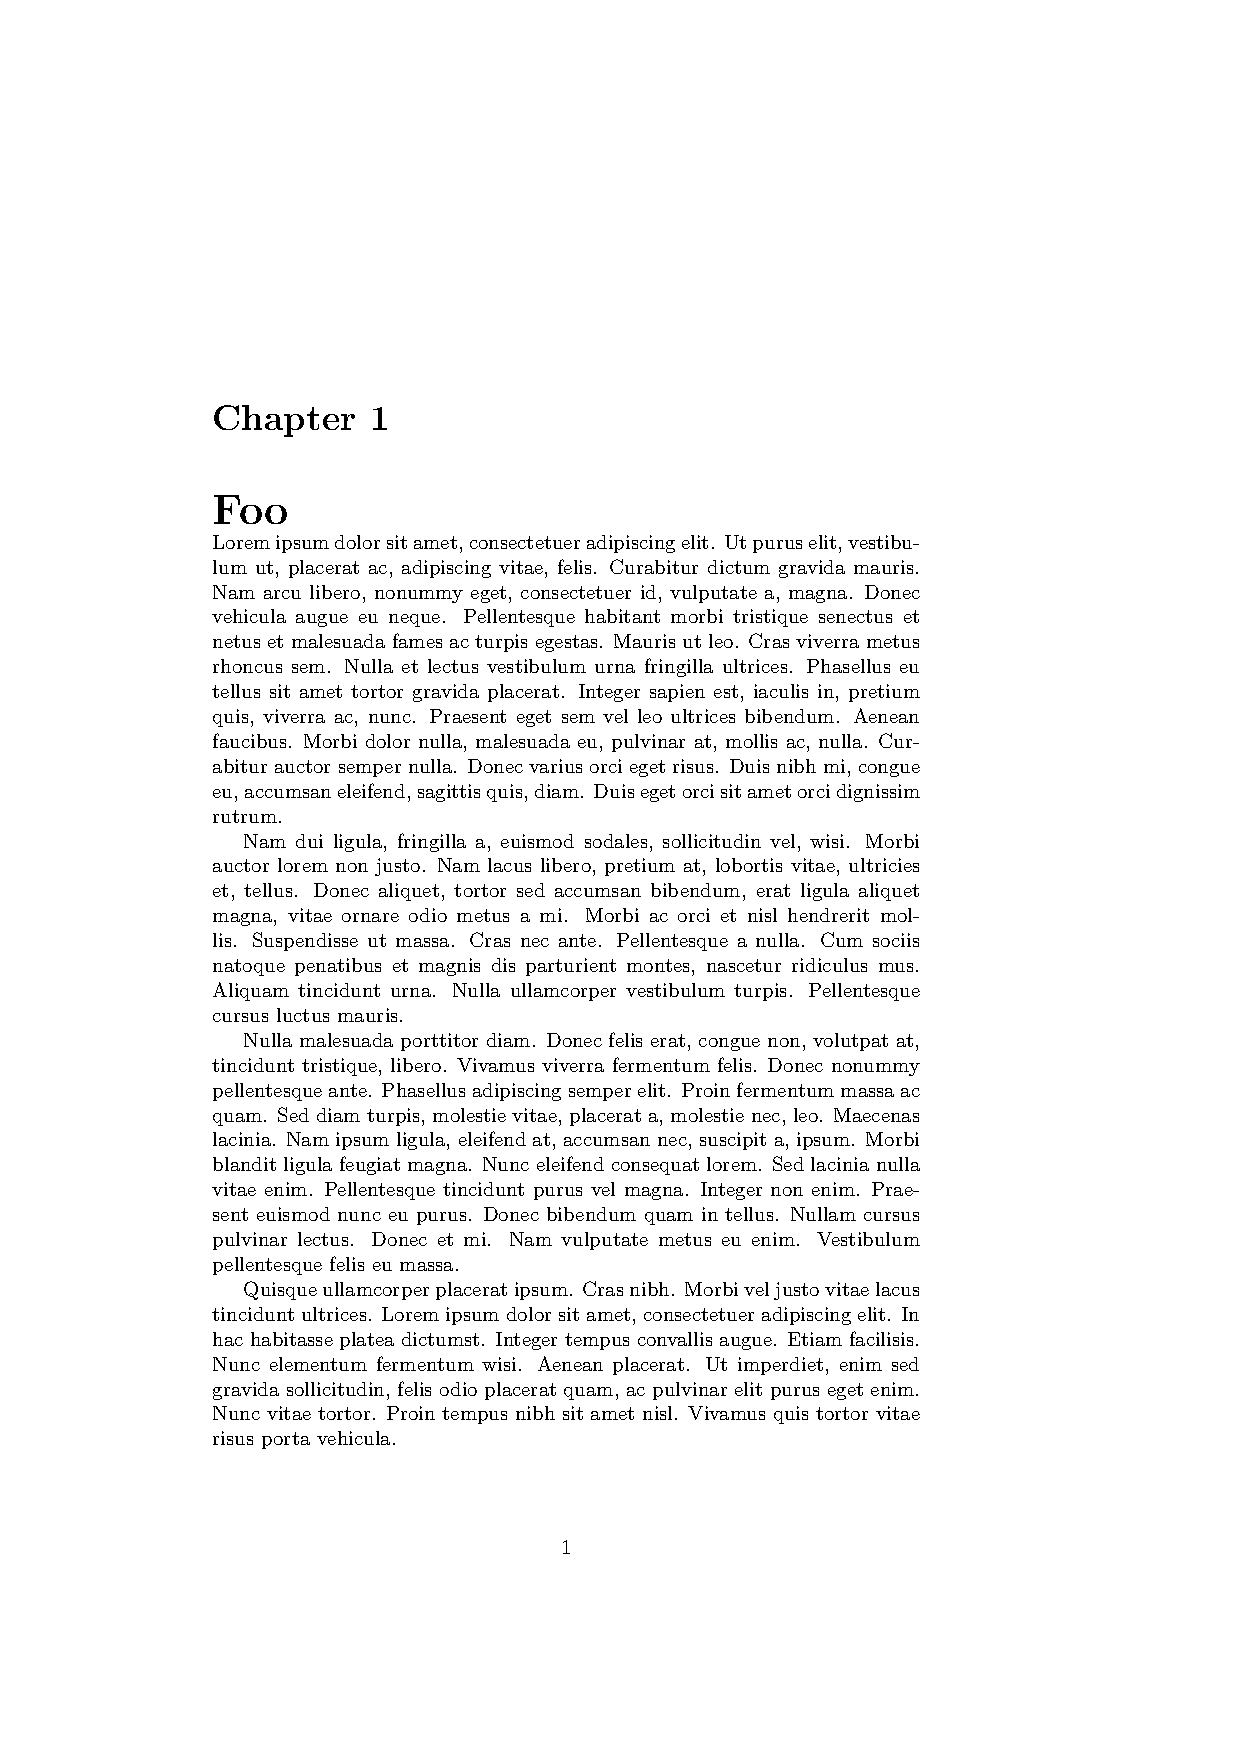
\includegraphics[frame,page=1,width=0.8\linewidth]{examples/afterchaptertitle-2}
        \end{center}
      \end{column}
    \end{columns}

    \onslide<2>
    \begin{columns}
      \begin{column}{0.5\textwidth}
        \begin{latexcode}
          \setlength\afterchapskip{40pt}
        \end{latexcode}
        \begin{center}
          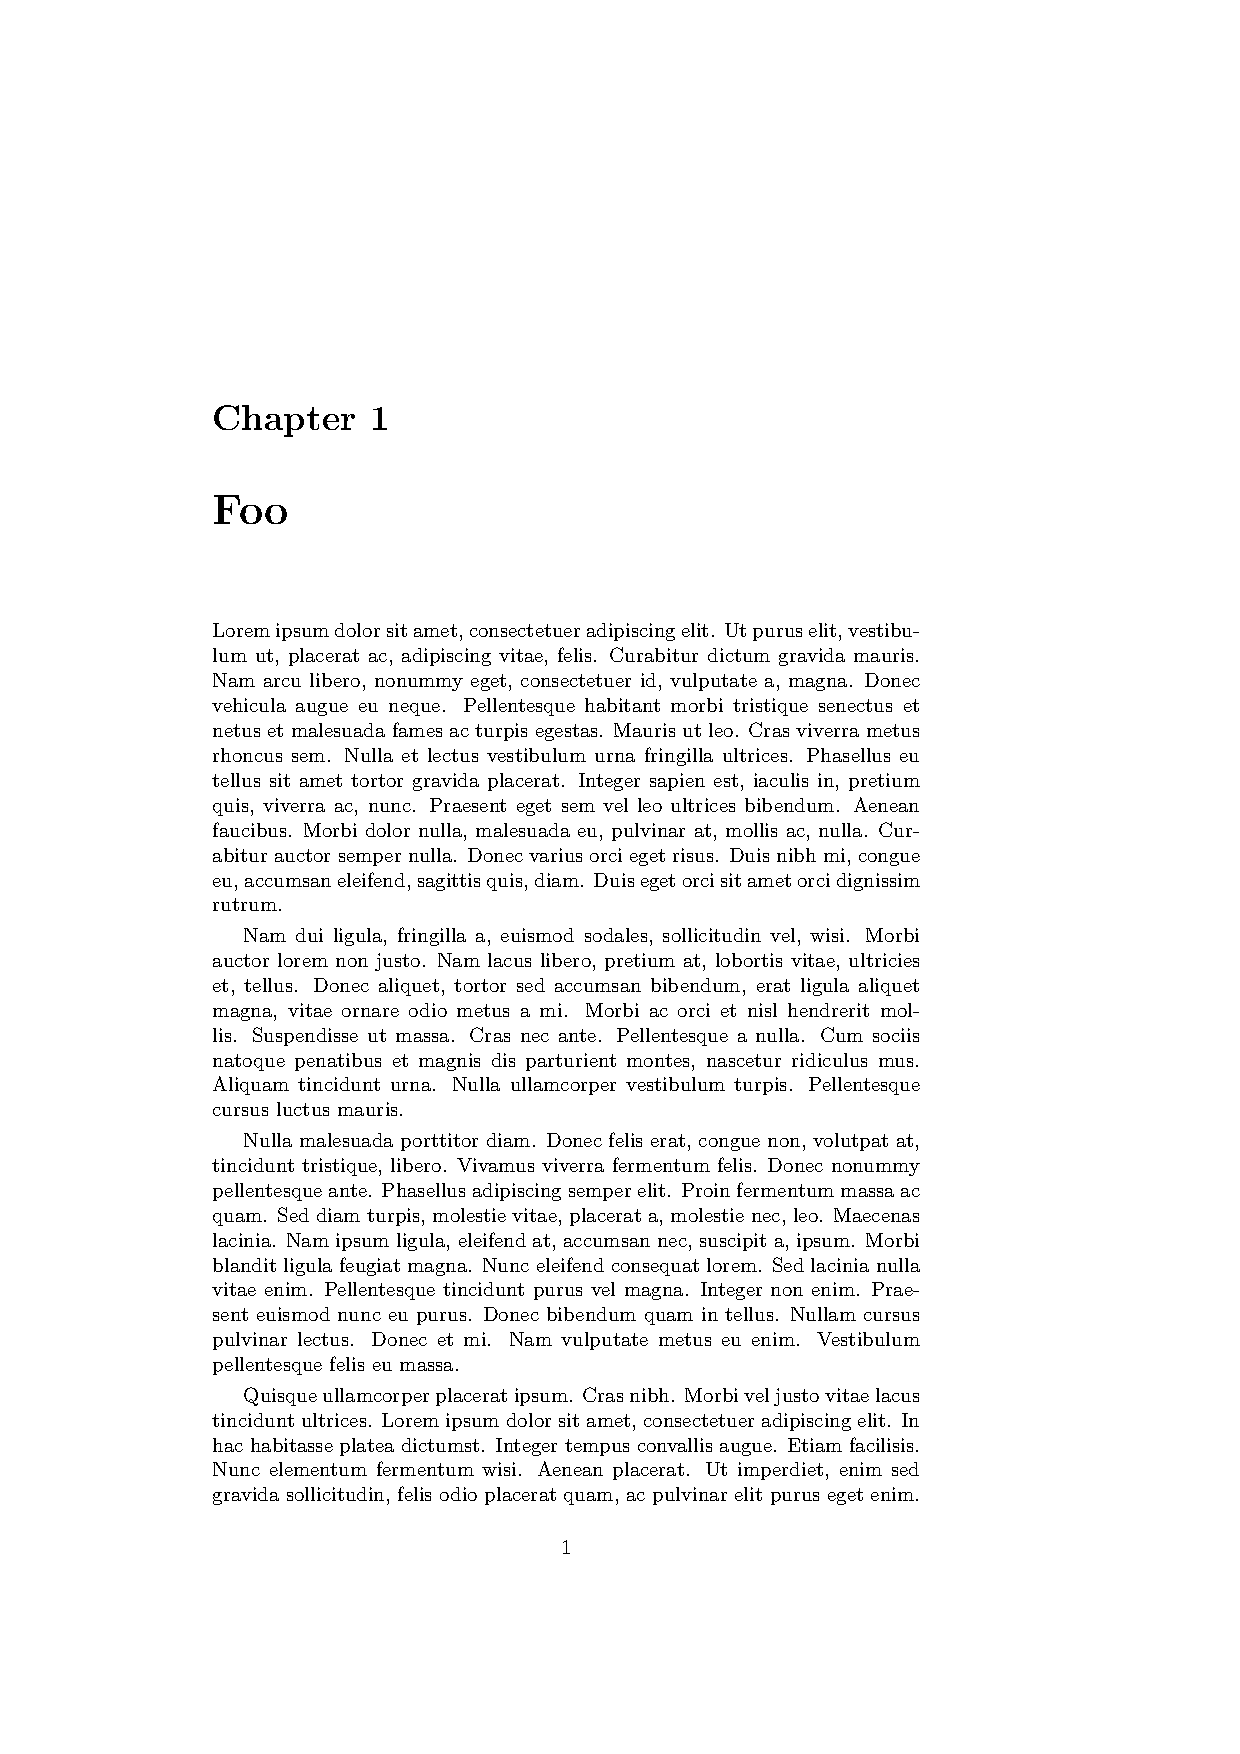
\includegraphics[frame,page=1,width=0.8\linewidth]{examples/afterchaptertitle}
        \end{center}
      \end{column}

      \begin{column}{0.5\textwidth}
        \begin{minted}[mathescape,
                       escapeinside=||,
                       autogobble,
                       linenos,
                       numbersep=5pt,
                       frame=single,
                       fontsize=\tiny]{latex}
          \renewcommand*{\afterchaptertitle}{\par\nobreak\vskip 0pt}|\vphantom{\LARGE a}|
        \end{minted}
        \begin{center}
          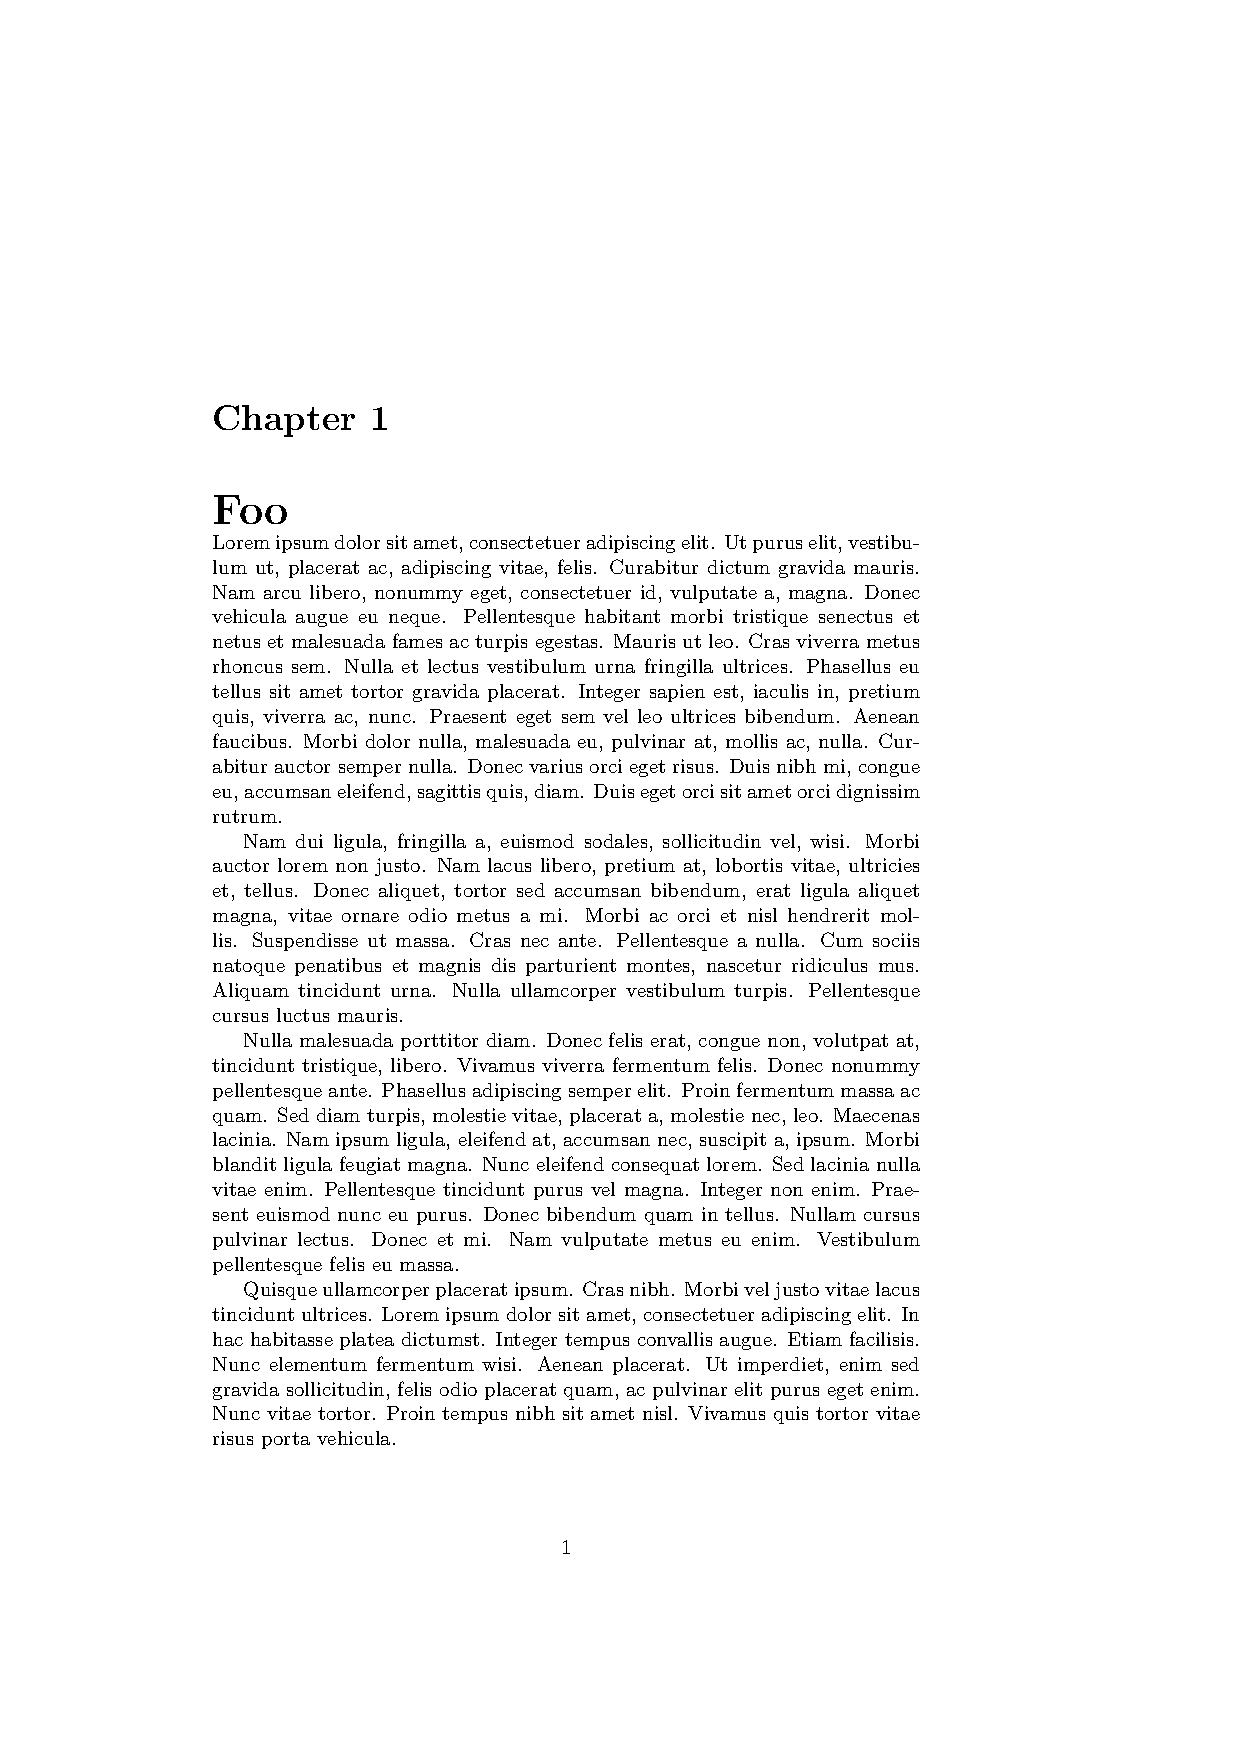
\includegraphics[frame,page=1,width=0.8\linewidth]{examples/afterchaptertitle-3}
        \end{center}
      \end{column}
    \end{columns}
  \end{overprint}
\end{frame}


\section{Case Study}

\begin{frame}[fragile]{Griffiths: Introduction to Electrodynamics}
  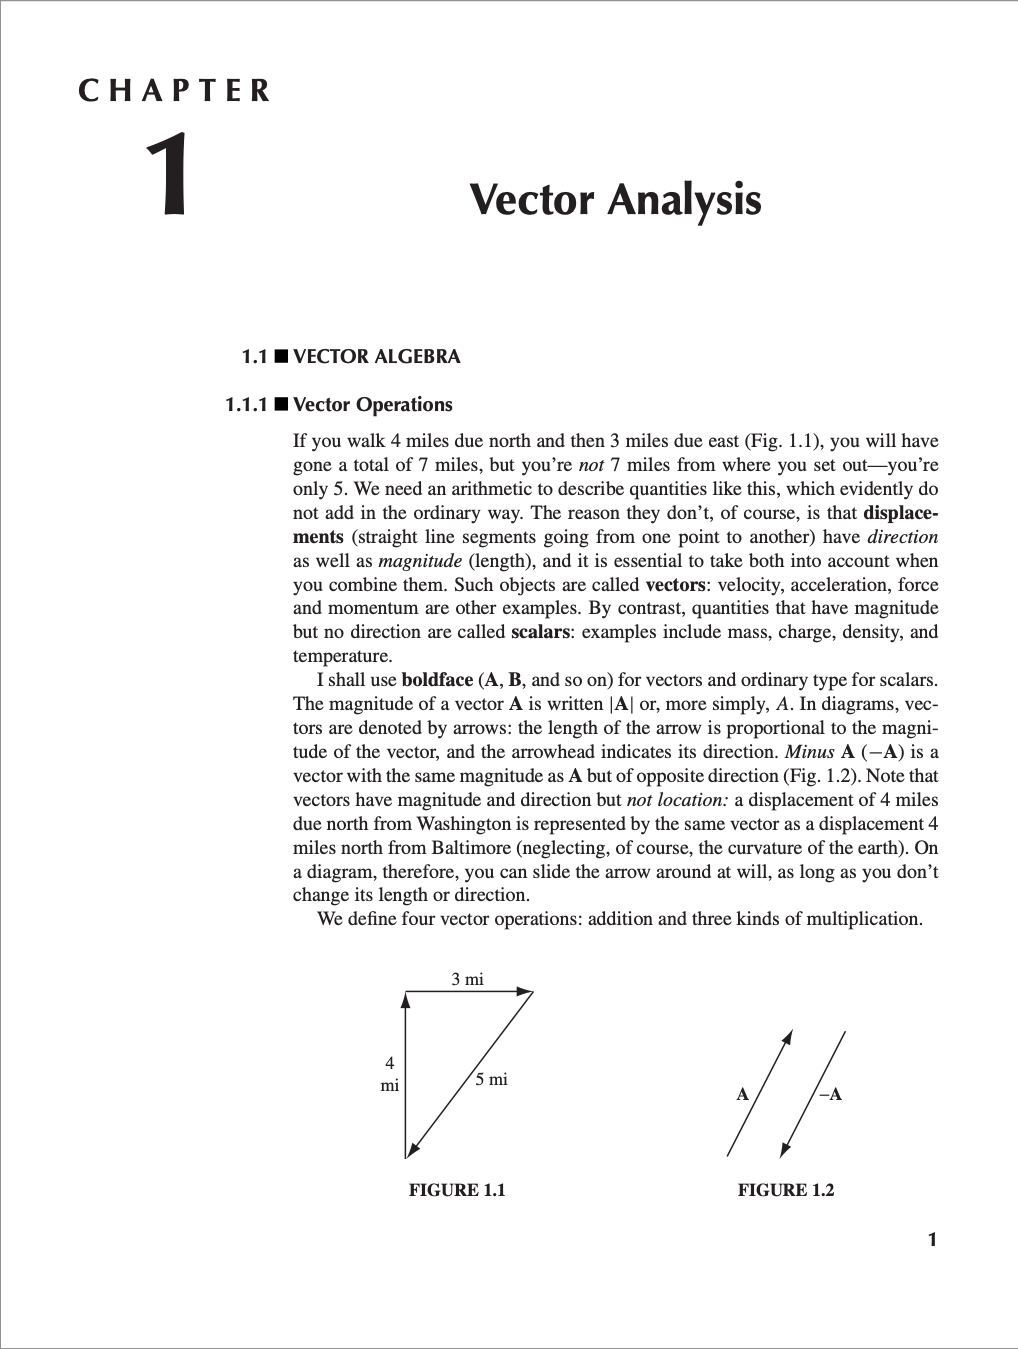
\includegraphics[frame,width=0.4\textwidth]{examples/griffiths}
\end{frame}
\end{document}
